\protect\hypertarget{titlepage.xhtml}{}{}

\protect\hypertarget{index_split_000.html}{}{}

NO. 6 \textbar{} Atsuko Asano

Volume 9 + Extra

\emph{So this was No. 6.}

\emph{This was Elyurias.}

\hypertarget{index_split_000.htmlux5cux23calibre_pb_0}{}

\protect\hypertarget{index_split_001.html}{}{}

\hypertarget{index_split_001.htmlux5cux23calibre_pb_0}{}

\hypertarget{index_split_001.htmlux5cux23calibre_toc_2}{%
\subsection{CHAPTER 1}\label{index_split_001.htmlux5cux23calibre_toc_2}}

\subsubsection{That which I say I saw}

\emph{Gracious my lord,}

\emph{I should report that which I say I saw,}

\emph{But know not how to do it.}

\emph{-Macbeth, Act V Scene V}

They were falling. Falling, almost straight down.

It was faster than anything Shion had imagined. He knew it was
impossible, but he heard the sound of the wind. It was the same wind
from that stormy night.

It was September 7, 2013―Shion's twelfth birthday. The Holy City of No.
6 had been directly hit by a hurricane. The rain was pounding on the
ground, and the wind was roaring. The trees in his yard careened wildly,
and leafy branches broke off and whipped through the air. It was an
extremely large and severe hurricane, a kind not seen in recent years,
but he was sure that no one living in Chronos felt threatened or
anxious. Shion and his mother, Karan, had been the same.

This was No. 6. A utopian city, the results of human wisdom and
cutting-edge technology. And in that utopia, Chronos was in the highest
ranks among the luxury residences, a town where only the chosen ones
were allowed to live. Mere natural disasters could not disturb it.

Everyone had believed so without a doubt. They had been allowed to
believe otherwise.

That stormy night, I opened my window.

Why? he sometimes thought. Why did I open that window? Was it because I
was excited at nature's madness, and I was stimulated, or I was stirred
by a violent impulse―was that it? I certainly did open the window, and I
yelled. I screamed as if I were pouring out all of the ferocity inside
me. If I didn't scream, I felt like I would shatter to bits. In my own
way, I felt a fear that I would be entrapped and tamed into domesticity
by No. 6.

A vague fear―maybe something that you wouldn't be acquainted with,
Nezumi.

I felt like I was suffocating. I was scared. I wanted to scream.

That was why I opened the window―wasn't it?

No.

That's not it.

You called to me.

I heard that voice―your voice―calling me.

It ducked through the wind, tore through the rain, and came to me.

You called me, and I was called by you.

That's why I opened the window. I flung it open wide to the outdoors.

I extended my arms in search of you.

Would you laugh? Would that breathtaking smile cross your face as you
sneer at me? Would you shake your head with exasperation in that
graceful way of yours?

'Meaningless fancies. An intolerable mass of self-consciousness, like a
half-baked artist's work'―would you spit those words at me? You probably
would. Go on and laugh. You can dismiss them as my delusions; I don't
care.

But it's the truth.

You called me, and I listened. I reached out, and you caught my arm. I
opened the window so I could meet you.

That's our truth, Nezumi.

A noise was ringing in his ears. It wasn't the whirl of the wind. It was
the sound of sliding through a plastic tube. But what if this tube was
not a garbage chute, but a steep slope that led straight to Hell?

Suddenly his consciousness began to fade. All the wounds he had suffered
on his entire body grew hot and throbbed. The strength left him.

Going to Hell doesn't seem so bad when it's with you. Should I stop
resisting, then? Why don't I just give up on struggling, on fighting, on
wanting to live?

If I let myself black out now, I'll be free from this pain, this
weariness.

Shion closed his eyes. Darkness fanned out before him.

Just like this... just like this....

"Ugh," Nezumi groaned softly. It stabbed Shion's eardrums. Like
lightning flaring up in a night sky, it tore the darkness away from his
consciousness.

Damnit. Shion bit his lip and inflicted pain on himself. He scolded
himself severely. You bastard, what were you thinking? You can't give up
now. Live. Survive. We have a place to return to, and we have to get
there in one piece.

He had made that vow. He had vowed to himself that he would protect
Nezumi through to the end, and survive this ordeal together.

His hand slipped. Nezumi's blood was caked on his palms. A black mouse
leapt out of his pocket and ran along the garbage chute wall. It wasn't
falling; it was definitely running.

Tsukiyo, I'm counting on you. Tell Inukashi that we're alive.

Shion jammed both feet against the wall and gritted his teeth. He
focused all the strength in his body on his legs. His bones creaked.
Their falling speed decreased somewhat. His bones continued to creak as
if they were screaming from the pain.

Damnit, I won't give in yet. Shion chewed his lip still harder. He did
not taste the blood. His tongue was already numbed to its rusty metallic
taste.

Inukashi―Inukashi, help us.

Inukashi!

Rikiga fell into a fit of coughing. He recovered and breathed raggedly.

"Inukashi, I can't do it anymore. I'm at my limit."

"Limit of what?" Inukashi said tersely.

"I can't breathe. Are you planning on suffocating me like this?"

"What good is it to me if I suffocate you, old man? You gonna leave me a
giant inheritance? The most you'd probably leave behind is a pile of
empty booze bottles."

"Hmph. See if I even leave you that."

But even while griping, Rikiga did not try to flee. He was still
stacking mattresses under the opening of the garbage chute. With each
mattress he stacked, he had a coughing fit, gasped and wheezed, and
griped some more.

Smoke had saturated the hygiene management room. The collection area was
no exception; it was almost engulfed by thick, grey smoke. The dogs lay
low on their bellies, their breathing hushed. Even the little mice who
had been squeaking clamorously at each other were now huddled
motionless.

The limit―Rikiga was right, the limit was near. Inukashi himself was
choking on the smoke, and the air wasn't passing through his throat
well. His heart pounded frantically.

It hurts.

The air is stuck in my throat.

But he was not miserable. He was not in despair. On the contrary, a part
of his heart was pounding, soaring in anticipation.

What is this smoke? This hot air that blows at me from time to time? The
restless buzz that comes with its snarl?

A clear precursor to destruction. The Correctional Facility is raising
its last dying shriek.

Many times Inukashi felt like barking out of excitement. He wanted to
bark and howl until his throat trembled. Just once, he opened his mouth
wide, but he only choked on the smoke that rushed into his mouth.

He licked his lips while carrying the mattresses. If I can't bark, the
least I can do is lick my chops.

What he thought was absolute was crumbling before his eyes.

Will you look at that. Is that what life is, Nezumi? Shion? If it is,
that means you guys taught me what it is to be alive. You never know
what happens. There's nothing absolute about what humans create.

I won't thank you; you guys have caused me too much hassle. You'll never
hear a word of thanks come out of my mouth.

But I owe you praise. I'll give you my best compliments. I'm actually
impressed that you guys turned out as decent as my dogs are. You guys
are really something. I have new regard for you. I'm impressed―just a
tiny bit.

The smoke assaulted his eyes, his throat, and his nasal passage. A tear
rolled down his cheek. It was just the smoke stinging his eyes.

You come back, you hear me? If you don't, I can't praise you. Hurry,
hurry, while my breath can still last me. Hurry.

Inukashi! Someone called him. He whirled around. Rikiga was kneeling on
the floor. He was holding a white cloth to his mouth, and coughs were
racking his bent back.

"Call me?"

"―What?"

"Did you call me, old man?"

"What would I... do that for?" Rikiga wheezed. "You want me to... give
you one last kiss or something?"

"Knock it off. That's creepy, even for a joke."

"I'm... past the point of... caring whether it's creepy. Really, I
can't... stand this anymore..."

"That's a shame. My heart goes out to you, man. But it's a bit too late
to repent. A man as corrupted as you isn't gonna get any closer to
Heaven, no matter how hard you try."

"Damnit... still smart-mouthing me... are you?"

Explosions. Smoke pouring into the air. The dog with patched fur raised
its head. Terror swam in its eyes. But the dogs did not move. They did
not try to flee.

They're waiting for my orders. They were waiting for Inukashi's command,
fighting their fear of death. Dogs never abandoned their master. They
never betrayed him.

I can't murder them like this.

"Go." Inukashi pointed at the entrance door. "Escape by yourselves."

But the dogs did not get to their feet. They remained lying on their
stomachs, watching Inukashi.

"What? I'm telling you to leave. Get out of here, quickly." He met the
eyes of the patched dog. Its eyes were serene. The shadow of fear that
had crossed his eyes moments ago was wiped cleanly away.

"I see..." You won't move if your master doesn't.

"Aren't you gonna... tell me?" Rikiga coughed and wheezed. "Aren't you
gonna... tell me to run?"

"You? You can get the hell out of here if you want to. You wouldn't be
any use if you stayed."

"Inukashi."

"What?"

"Do you... plan to die here?"

"Die? Why would I?"

"There's barely any... chance that those two... Shion and Eve... are
going to come back. If you're gonna gamble on that slim chance... if
you're gonna gamble and choose to stay... that's like killing yourself."

No way. Heaven and earth can turn upside-down, but I'm never gonna kill
myself. I'd be missing the spectacle of a lifetime. The destruction of
the Correctional Facility was only the beginning. It was only the
preamble. The devastation of No. 6 itself was what came next.

No. 6 was falling apart.

I'll get to see the very moment with my own eyes. And you're telling me
I intend to die? You must be kidding me. You bet I'll live to see No.
6's last. I'll thoroughly enjoy its final act.

Heh heh heh.

Lighthearted laughter rang at his ear. No, it was in his ear―inside his
head. Someone was laughing. It was carefree and joyful, yet an icy
laughter.

"Who is it?"

His gaze darted about instinctively and caught a small black shadow
passing by.

A bug?

The shadow was soon swallowed up by the smoke as it disappeared. The
laughter ceased. Were they both hallucinations? There's no way a bug
could be flying around in this smoke.

Shiver. A chill ran down his spine.

Screech, screech, chit-chit!

Cheep-cheep-cheep-cheep-cheep. Squeak!

Suddenly, the mice began to cause a commotion. They raised their voices
again, but much higher this time, and dashed around on top of the
mattresses.

Inukashi held his breath.

A small object came tumbling out of the chute. It was not trash. It was
a small black mouse.

"Tsukiyo." Inukashi tried calling it. The black mouse flew through the
air; it leapt straight for Inukashi. It latched onto Inukashi's hastily
extended arm, and squeaked insistently.

Cheep cheep cheep cheep! Cheep cheep cheep cheep!

It was Tsukiyo; there was no doubt about it. It was the same little
mouse that Inukashi himself had commanded to go to Nezumi. His blood
stirred. His body grew hot.

"Wake up, old man."

"Eh?"

Rikiga blinked feebly, still squatted on the ground. His eyes were
bleary and red. His face was sooty, his hair was mussed, and he looked
like he had aged a good decade.

"They're coming back."

"Eh?"

"Coming back. Hold onto the mattresses."

"R-Right." Rikiga got to his feet in a surprisingly swift move.

The wind was howling.

As Inukashi and Rikiga held the mattresses down, they felt a heavy
impact almost simultaneously. The mattress sank, almost sending
Inukashi's slender frame flying. He summoned all the strength in his
body to cling onto the mattress.

He had instinctively closed his eyes, but now he opened them carefully.
He saw two bodies lying in a heap.

"Shion, Eve!" Rikiga yelled before Inukashi could speak. "You alright?
Hey! You alright?"

"Gh..." Shion's arm jerked. A part of his white hair was dyed with his
blood. Blood was streaming from his shoulder and his leg. His clothes
were torn, ripped, and hanging in places. Inukashi couldn't tell if the
dark flecks all over his clothes were from blood or the trash in the
chute.

Horrible. Inukashi kept his eyes wide open as he swallowed his spit,
which smelled like smoke. You guys are a mess. I think even the undead
would look a bit better crawling out of their graves.

"...Inukashi." Shion lifted himself up and turned his face to Inukashi.
His cheeks were streaked―whether it was with sweat or tears, he didn't
know, but they engraved prominent marks on his skin.

"Shion, you're alive." You made it back alive.

"Inukashi, save Nezumi..."

"Nezumi? What about him? What―" Inukashi was barely able to hold in the
scream that threatened to burst from his throat.

Nezumi was lying on the mattress, totally still and unmoving. His
clothes were soiled reddish-black from his shoulder to his chest, and he
gave off the smell of blood.

"Nezumi, hey, what's wrong?" Inukashi asked tentatively, but there was
no answer. On his pale, bloodless face, only his lips were vividly red.
To Inukashi, they did not look human at all. Nezumi had always had a
face that was somewhat otherworldly, but the face in front of him was
one of a doll. A skillfully and meticulously crafted piece.

But dolls don't bleed.

"To the hospital―hurry," Shion screamed, as if wringing the voice from
his throat. Explosions rocked the foundations of the building. The whole
room shook with its impact. A draft was coming in from somewhere, and
the smoke wavered and thinned slightly. The shaking did not stop.

"We need to get out of here! This place is coming down!" Rikiga yelled
as he wrenched Nezumi away from Shion's arms. He slung the boy over his
shoulder.

"Shion, can you run on your own?"

"I can."

"Right, then run. Get outside."

One more sound, more violent than before, rang out, and the door to the
Correctional Facility was blasted away.

"Run, run! This place won't hold much longer!"

Rikiga broke into a run, bearing Nezumi. Tsukiyo dove into Shion's
pocket, and the two mice, Hamlet and Cravat, leapt onto a dog's back.

"Get out, goddamnit! Get out of here!" Rikiga's bellows slammed into
him.

His back was blistering hot. Inukashi turned around to the flames
filling his vision. Beyond the blown-open door, the Correctional
Facility was burning.

The door blew apart? Wasn't the door between the Correctional Facility
and the Hygiene Management Room supposed to be made of some special
alloy that even a small missile couldn't penetrate? And it's been blown
apart like it's nothing?

For less than half a second, he stood stupefied. Flames slithered. A
fire-coloured monster was writhing on the floor. It writhed and twisted
towards the corpse of the black dog and swallowed it whole. It was the
same dog that had been shot to death protecting Inukashi, but Inukashi
was unable to give it a proper burial.

Sorry.

"Inukashi, hurry!" Shion grabbed his arm.

"Get out, get out! We have to get out of here!" Rikiga continued to
bellow. He seemed to be turning his yelling into energy to move forward.
Inukashi was pushed along by the heat and the hot air from behind, and
quite literally stumbled into the outdoors. Fresh air flowed into his
body.

Oh, I can finally breathe.

"Not yet. We can't stop yet. Keep running." Shion's grip tightened.
Inukashi was dragged along by his arm. The gravel crunched under his
feet.

"Ow! Shion, that hurts! Stop―" Inukashi abruptly closed his mouth. His
eyes had met with Shion's.

His eyes, dark with a wash of purple, were the same as always. They were
completely unchanged. They were bloodshot, and the eyelids were swollen,
but they were Shion's eyes.

Yet Inukashi closed his mouth and felt his body stiffen. He did not know
why. The boy in front of him telling him to run seemed a complete
stranger. He was someone Inukashi did not know.

No. Those aren't Shion's eyes. Shion, what's gotten into you?

But the confusion and foreboding vanished in an instant. Shion was
right―he could not fall to his knees just yet. His instincts sounded the
alarm. This physical sensation was much more reliable than any
cutting-edge security device.

Get out of here, run. Get out of here.

Inukashi leapt to his feet, and ran as fast as he could. From behind, he
could hear the roar of a beast. Yes, those were not just explosions. A
monster was baying. It was raving madly.

Get out of here, run. Get out of here.

Run and survive.

Tsukiyo had crawled out of Shion's pocket and was clinging onto his
neck. It had opened its tiny round eyes as wide as it could, and was
staring over at Inukashi.

You're kinda cute.

Dogs' eyes and mice's eyes were alike, and all such innocent beings were
loveable. Inukashi thought of Shionn. He had not forgotten about him for
a moment. He had only pushed the infant to a corner of his heart so as
not to remember him when he was not supposed to.

Shionn was innocence itself. He was so small, yet he had so much inside
him.

The dogs are probably managing alright. I left him with a dog that's
birthed and raised a ton of her own puppies. Apart from her, there are a
few other caring females in waiting. He's probably sleeping right now,
protected by his loving nurse.

"Shionn, my baby," he murmured. Just then, Rikiga, who had been running
in front of him, disappeared. He heard a shout, and the sound of a body
falling over.

"Whoa!" Shion tripped over Rikiga's fallen body. In turn, Inukashi's
feet were swept from under him by Shion, and he was slammed to the
ground. The pain racked him to his very core.

He could not speak. Lying on his stomach on the ground, he could only
draw strained breaths. He could feel the frozen ground on his cheek. It
was soothing. It had not the iciness of winter, but a cold that
harboured a faint hint of warmth and softness.

Spring was coming. A late spring was starting to arrive in the West
Block.

No. 6 was probably fully furnished with flowering parks and streets
lined with cherry blossom trees, but one would be hard-pressed to find
even a single flowering tree in the West Block. But the weeds growing on
the shoulders of the road faithfully opened their petals year after
year. Flowers usually sparked no interest or intrigue in Inukashi since
they were not edible, but once in a while they pulled at his
heartstrings.

Oh, I've lived through another winter, he would think. Then, for a
fleeting instant, in the back of his mind he saw faces of those who had
frozen to death that winter―the old beggar lady he had been familiar
with; the man who had hung around the ruins for a good while; the woman
who was so emaciated, it was hard to tell her age―but they disappeared
as quickly as they had come.

Spring was coming. Would those flowers bloom again on the side of the
road?

"Nezumi," Shion gasped. He lifted himself up, and crawled over to
Nezumi's side. "Nezumi, Nezumi. Can you hear me? Nezumi―"

Inukashi also lifted himself up. They were lying in the shadow of some
shrubbery. When was it that he had hidden himself here, witnessing
Getsuyaku being shot to death?

It felt like it had happened only minutes ago, but at the same time a
thousand years back.

"Nezumi, open your eyes. We're out. We were able to get out."

Shion's voice sounded like the wind that whistled through the ruins. It
was mournful. It froze the hearts and ears of those who listened.

Inukashi peered over Shion's shoulder at Nezumi's face, and compressed
his lips into a hard line.

Is he dead? The statement pushed his lip up and threatened to spill out.
Shion, is Nezumi dead? Or is he just acting? Who's he playing? Macbeth,
Hamlet, or some other weird name that you guys used to mention?

Hey, Shion. Don't tell me Nezumi is really―

"Gh―" Nezumi's eyelashes trembled very slightly.

"He's alive," Shion shouted as he lifted Nezumi in his arms. "He's
alive! Hurry, to the hospital!"

Yeah, you're sure alive. You can't trick me, Nezumi. There's no way you
would be wiped out that easily.

"Old man." Inukashi called to Rikiga, who was squatting on the ground.
His car was parked beyond the shrubs. It was a piece of junk, a step
away from scrap metal, but it could still chug along with a couple
passengers. They had taken this gasoline-fuelled car to get here, after
all.

"Old man, hurry up."

"―I know, but―"

Rikiga held a hand to his mouth, and stuck his head into the bushes. The
sound of retching reached them.

"Dumbass! This is no time to be puking! Hurry the hell up, come on!"

Inukashi grabbed the man by the belt of his trousers and dragged him out
of the bushes. Almost as if in answer, an even larger flame burst out of
the window of the Correctional Facility. It threw a bright light on the
surroundings. Black smoke formed a thick stream as it rose into the sky.
It engulfed and blacked out the stars.

Can you see these flames from No. 6, too? What would West Block
residents be thinking right now as they watch the flames burning the
night up?

Look at it, it's falling. A place that used to mean Hell for us is
collapsing. It's gonna be wiped out, just like that, even quicker than
our marketplace.

Rikiga got to his feet unsteadily. He wiped his mouth with the back of
his hand, and wiped the sweat on his brow while he was at it.

"Why do I... have to go through this? Besides, you know, I―"

"Enough crap," Inukashi interrupted. "No one's listening. If you've got
time to bitch and moan, get the car moving."

"Moving where?" Rikiga snarled. "Eh? Answer me this, Inukashi. Where are
we going to take someone who's hurt so badly he's as good as dead?
Answer me, I'd like to see you try! If you can give me an answer, boy,
I'll take you wherever the hell you want."

Inukashi drew his chin back and fell silent. He could not answer.

He was not intimidated by Rikiga's angry outburst. He genuinely did not
know. 'To the hospital,' Shion had said, but there were no medical
facilities in the West Block. There were seedy witch doctors and
questionable medicine shops, to be sure, but they had all been blown
clean off their foundations during the Hunt. But even if they were still
around, they would probably not have been of much use.

Rikiga continued his furious tirade.

"Someone who's bled this much is going to need a decent amount of
medical equipment. Where do you suggest we find that, huh? Nowhere here,
for sure. You can scour the whole West Block and you won't find a single
damn syringe. You should know that best, Inukashi."

Inukashi looked down at Nezumi. His lips were parted slightly. He was
breathing. But―

This is the end, huh? The strength withered in his legs, and he felt
like he would collapse. This is it, Nezumi. There's nothing more we can
do.

"There is." Shion stood up. "There is a hospital."

Inukashi and Rikiga turned to each other. They peered into each other's
eyes.

"Hospital―? Where?" Rikiga asked in a hoarse, scratchy voice. Shion's
gaze slid to the side. On the other end of it was the special alloy
wall, illuminated brightly by the flames.

"Inside."

"No. 6!" Inukashi and Rikiga's voices overlapped.

"Yes. We'll find plenty of hospitals there."

"That's absurd!" Rikiga blurted. "How are we going to get inside? My car
won't even be able to pass the gates. They'll register it as a
suspicious vehicle and it'll get blown up within a few metres of even
entering. Impossible. Absolutely impossible. Wait, I know! Shion, how
did you escape from No. 6? Can't we go back in that way?"

Inukashi almost interjected in agreement. If Shion had come out that
way, perhaps he could get back in through it. That old man is a quick
thinker once the alcohol's gone out of him.

But Shion shook his head firmly.

"We can't do that. That would take too much time. And Nezumi wouldn't
last on the strength he has left. We have an hour―we need to get him to
the hospital within an hour..."

"But how are we going to manoeuvre through the gates?"

"We don't need to."

"What?"

"The Correctional Facility is destroyed. All its functions have shut
down. That means the gates mostly likely aren't operating, either."

"You're planning to enter No. 6 through the Correctional Facility's
private gates?"

"Yes."

"Shion, you... do you know where the Correctional Facility's gates are?"

"I don't know for sure. I've heard, though, that they're directly
connected to the Correctional Facility."

Rikiga's throat contracted as he swallowed his saliva. Inukashi found
himself doing the same. The back of his throat burned from the smoke.

"You're right." Rikiga's voice grew even more hoarse. "You're absolutely
right. It's directly connected. About a hundred metres beyond the gates,
you'll find the back entrance of the Correctional Facility. That's where
you two were carried through during the Hunt. But you probably couldn't
see anything from inside the cargo container you were loaded into."

Inukashi realized he had unknowingly clenched his hand into a fist,
listening to Shion and Rikiga's conversation.

Getsuyaku had also been coming and going through those gates. Inukashi
had heard him complain countless times about being treated the same as
prisoners. Inukashi had given the man an offhand answer.

"Prisoners are killed once they get caught. They'll never come back out
through those gates again. But you're coming and going through them
every day. Not to mention you're getting paid to do it. That's way
different from being a prisoner."

"Well, I guess, now that you mention it. I wouldn't be able to go home
if I were just a prisoner, huh," Getsuyaku had shrugged and smiled
ruefully.

But in the end, he was the same. He was shot dead in the blink of an
eye, just the same as a prisoner. Even worse―like an insect.

Inukashi remembered Getsuyaku's rueful smile. He closed his fist more
tightly.

"Then we can take the car to the gate from here, right?" Shion asked.

"We can if there are no obstacles along the way. No one is crazy enough
to get close to the Correctional Facility now, apart from you lot."

"Rikiga-san, lend me the keys to your car, please."

Shion extended his scratched and bloody hand. Rikiga's face twisted
visibly. Deep creases appeared between his eyebrows.

"What are you going to do with them?"

"I'm going to drive. You two can stay behind. The keys, quickly."

"Bullshit!" Rikiga bellowed angrily again. "Have your eyes rotted and
fallen out? Don't you see those flames? You idiot!"

The Correctional Facility barely remained standing, spewing flames and
black smoke. The alarms that had been ringing so loudly had died out
somewhere along the way, and only the ferocious wind sounded as it was
drawn in by the flames.

"We've barely gotten out of the Correctional Facility in one piece, and
you're going to prance right back in?" Rikiga said incredulously. "This
is no time for jokes. How many lives do you think you have?"

"I don't plan on going inside. The gates are outside of it."

"A hundred metres away. Only a hundred metres. The gates aren't a safe
zone, you know."

"That's why I'm going. Usually we wouldn't be able to get through, but
right now, the gates are nothing but an opening."

"The car runs on gasoline. If you happen to drive into fire and it
catches―"

"Hand it over," Shion commanded in a low voice, cutting through Rikiga's
yelling. Commanded. That was indeed how the words came out. Shion had
neither snapped, nor yelled harshly. On the contrary, it was a quiet and
heavy utterance.

Rikiga retreated half a step.

"Hand over the keys."

It was the voice of a ruler giving orders to his subject―it was
unmistakable.

Rikiga rummaged through his pocket and extracted a worn silver keyring.
His fingertips were trembling.

"...Stop it," said a voice even lower than Shion's. To Inukashi it
seemed to spring from the depths of the earth. A chill ran through his
spine. Nezumi had slowly lifted himself up.

"That's enough. Stop it."

Inukashi could hear his words clearly.

Nezumi's voice. Nezumi could use ten, twenty different voices, but what
Inukashi's ears had caught was unmistakably Nezumi's natural voice.

"Don't... stay away, Shion."

Shion did not answer. He did not even try to look at Nezumi. Instead, he
bowed his head to Rikiga.

"Rikiga-san, please. Give me the keys. Please, I'm begging you." It was
not an order, but a plea.

This was the Shion that Inukashi knew. Intelligent, gentle, faithful,
airheaded and clumsy Shion.~

"Just give it to him, old man," Inukashi said with a deep sigh. He
didn't know why he had sighed. There were a lot of things he couldn't
make sense of. He couldn't even understand himself.

"Shion, I'll go with ya." The words spilled out along with his sigh. He
surprised himself. Look at me. I'm so reluctant to put my life in
danger, I'm so desperate to survive, yet here I go saying 'I'll go with
you'. I can't believe myself sometimes. And what's worse is that it
isn't even a lie or bravado. I really mean it. I told him I'd go with
him, and I meant it. What on earth is wrong with me? I can't understand
myself. What's going on, what's going on, what's going on? Oh, hell.

"Fine." Rikiga clicked his tongue. "If that's what you want to do, then
do as you will. You guys probably aren't the type to listen to your
elders, anyway."

"Don't lump me in with the airheaded young master, man," Inukashi
protested. "But, oh well. There you have it. The votes are in and it's
two to one for driving into No. 6. That's that. Too bad, Nezumi."

"Three to one." Rikiga clenched the keys. "I'm coming along for the
ride."

Inukashi blinked and glanced at Rikiga. The man also blinked repeatedly,
his eyes ringed with soot, dirt and sweat.

What on earth is wrong with me? Why did I say something like that? And I
actually meant it, his facial expression seemed to say. Inukashi felt
like laughing and crying at the same time. What a weird feeling. He felt
scared, yet exhilarated. Dismal, yet optimistic. Your heart can be weird
like that.

"It's my precious car," Rikiga said. "I won't tolerate you trashing it.
Besides, I doubt you snot-faced kids would be able to drive. Young'uns
these days get better and better at mouthing off, but can't do anything
for themselves."

Rikiga mumbled complaint after complaint. It was most likely because he
would end up sighing if he didn't talk.

Rikiga's car was a minivan. It was dented everywhere, and the right side
mirror was bent. It was an outdated gasoline-fuelled model that could
easily have been displayed in a museum in No. 6.

But it had a sturdy frame, if anything. The engine also had a lot more
power than it looked. Being able to drive a car in the West Block was a
symbol of a certain level of wealth, and hence there was always a risk
of being ambushed by thieves on the road. Inukashi remembered listening
to Rikiga boast that for this reason, he had modified the car to be as
durable as a tank.

Inukashi sat in the passenger seat, while Shion sat in the back holding
Nezumi. The dogs climbed into the car last.

"Why do you have to bring your dogs? They'll stink up the car."

"They smell way better than your alcohol. My dogs are loyal to their
boss. They'll go wherever I go. Just like how these tiny mice are
faithful to their boss."

The mice were huddled together on the seat. They sat noiseless, as if
they had forgotten how to squeak.

"Dogs and mice, huh. That settles our destination, then: the zoo. Hmph,
what a fun drive this is going to be."

Rikiga turned the ignition. The engine sputtered comically, and the car
seemed to give itself a shake.

"Let's go. I'm going to floor the gas, so you better prepare
yourselves."

The car lurched forward. It continued to mount in speed as it made
straight for the Correctional Facility.

"Hey hey, old man. It seems like you're being a little reckless about
this."

"How can I not be? Look at what I'm doing. Damnit, what the hell am I
doing? Why the hell am I doing this?"

"Because you're in love with Eve, duh."

"What?"

The back gates to the Correctional Facility had been thrown open.
Perhaps some people had escaped through them. These gates had always
been tightly closed, refusing all who came near, but now it was open and
exposed. Flames spiralled up behind them, and the building played its
melody of destruction. Inukashi could hardly believe that this wasn't an
illusion.

Is this reality?

The gates to the Correctional Facility had opened, and the special alloy
door had been blown apart.

Things that were not supposed to be happening were happening. Things he
had believed would never happen―no, had been made to believe would not
happen―were inverted. There was no good or evil. No justice or
injustice.

This is reality.

The car veered around the back gates, nearly scraping against them, and
gained speed. Inukashi saw the security gates beyond.

"What!?" Rikiga yelled. "What did you just say, Inukashi?"

"You were totally into Eve, old man. You're still a passionate fan,
aren't you? You're head over heels. Or else you wouldn't be able to
sprint like that while holding him. Those were some good moves out there
on the field, risking your life. Bravo."

"Knock it off. Once we get to a medical clinic, the first thing I'll do
is sew that mouth shut. Sew in that rotten tongue of yours while I'm at
it."

"Why, that's just splendid. An honour of honours to be able to get
treated at a clinic in No. 6."

"Say all the crap you want!" Rikiga gripped the steering wheel.

Inukashi snapped his eyes open, and shrank back. The gate was
approaching at an astonishing speed. No, they were approaching it.

"It's burning," he murmured. He had resolved not to voice it; he had
restrained himself from putting anything he saw into words. But he could
not help it.

The gates were burning.

They were engulfed in flames. Small explosions, still not as large as
the ones in the Correctional Facility, were ringing out. Fragments of
glass and metal battered the car ruthlessly. Each time, the car made an
unnerving bump-bump sound. The sounds were like the car's screams
themselves.

It hurts. I'm scared. I'm gonna die.

"It's burning." Once he put it into words, terror gripped his whole
body. It was like the roots of his hair were standing on end. But one
point of curiosity slipped through the wave of fear washing over him,
and clung to Inukashi persistently.

How can it crumble so easily?

He understood that Shion and Nezumi had utterly destroyed the core of
the Correctional Facility. He was in awe at their accomplishment. But
there was something wrong with it. It happened too fast, too easily. Was
it always this fragile? Is it supposed to just collapse like that? He
did not think for a bit anymore that No. 6 was an absolute existence, or
an omnipotent ruler. It was the same as that special alloy door. It had
bent out of shape, crumbled, and now lay in a disgraceful mess.

But―but this is No. 6 we're talking about here. An artificial city, the
epitome of human intelligence and scientific technology. The
Correctional Facility is another No. 6 that's supported its darker
workings. It's No. 6's bastard child, an evil spawn that's a spitting
image of its parent.

Evil things often possessed evil powers. Couldn't it have stood its
ground somehow? Is it going to be defeated just like that, without a
choice?

Heh heh heh.

He heard it again. That lighthearted but terrifying laughter. It was
more frightening than the flames in front of him.

Inukashi screamed. Rikiga gave a shout beside him almost at the same
time. This one was from the fear of being on the brink.

"Ahhhhhh!!!"

They plunged into the wall of fire. The dogs continued to bark
incessantly. Inukashi did not close his eyes. He kept them open, and
watched the flames swallow them up. They were not a uniform colour. The
vermillion of sunset, the crimson of blood, the red of flowers all
blended together. They shone golden, then sank into a muddy red.

A part of the windshield shattered. Hot air blasted at them full-on in
the face. He smelled burning hair. The heat evaporated the moisture from
everything around them, and they began to shrivel up.

Oh, so we're gonna die here. So that's how it is, he thought. I'm going
to die with them after all. In the end, I'm just...

"Elyurias," said a voice from the back seat. Inukashi could not tell if
it was Shion's or Nezumi's. He did not know what the word meant. Was it
an incantation? It sounded too strange to be someone's last utterance.
But then again, they were always strange, weird, ridiculous people from
the beginning. This doesn't surprise me now, but... it's nagging at me.

Elyurias? What the hell is that?

His hair singed. His skin was being roasted. It was hot. Goddamnit, it's
hot.

The flames wavered. They wavered, and seemed to retreat just slightly.
The heat also receded just slightly, and he could breathe a little.

Huh? Why? Inukashi blinked. Are the flames retreating on their own? No
way. That's impossible. Absolutely impossible.

"We're out! Rikiga roared with laughter. He laughed as if he had gone
mad. "We're out! Take that, bastards! We're out safe! Ha, ha, ha ha ha
ha ha ha! Take that! We've done it! Ha ha ha ha ha ha!"

Tense laughter echoed inside the car.

Ha ha ha ha ha! Ha ha ha ha ha! Ha ha ha ha ha!

They had gotten through. He was right; they had certainly gotten
through.

The land around them wild and barren, with few grasses or trees. It was
no different from the West Block. But at least in this wasteland, there
was a straight, two-lane road. A lush, green forest probably awaited
them at the other end. In the dark, Inukashi could only make out a black
mass, but Inukashi's nose caught the rich, earthy smell of the trees.

Maintained roads and lush forests―all were things he could never see in
the West Block.

We've made it inside No. 6. I've stepped inside, for the first time in
my life.

"Look at that. That was quite something. Ha ha ha ha ha! Only natural
for Almighty Mr. Rikiga! I'm quite the hero. Ha ha ha ha ha, I did it!
Take that, bastards! Hooray for Mr. Rikiga, hip-hip-hooray! Ha ha ha ha
ha!"

Rikiga's voice cracked even more, and whined in a higher pitch. Inukashi
swept up a liquor bottle that had been lying at his feet, and knocked
Rikiga over the head.

"Ow! What was that for?"

"I went easy on you. Your head hasn't cracked open, now, has it?"

"Idiot! How dare you act like that to a hero!"

"I calmed your hysterical fit. That's really sad, old man. Even my dogs
and the mice are calmer than you. What's so heroic about what you did?
You went on a reckless joy ride, and you jumped through fire. That's it.
Ugh, for shame."

"Shut up. Can a dog or a mouse drive a car? I'd like to see them try.
You think you've got a right to say whatever you want―"

Once Rikiga finished yelling to his heart's content, he gave a great
sigh.

"Shion, what are we going to do now?" he said. "I have no idea what it's
like inside No. 6. I've been away for ten years."

Inukashi could feel Shion shift in his seat.

"Lost Town is just a little ways in from here. The outskirts of No. 6
are beyond that forest, and further beyond that are the central
districts. The forest is there to hide the walls from the citizens."

"I see. So they can go on living without being reminded all the time
that they're surrounded by a wall."

"Yes."

"And how about medical facilities? Where should we go?"

"Go straight through the forest. There will be a fork, and if you turn
right, there should be a small clinic."

"Will that be good enough? Eve's hurt pretty badly, isn't he?"

"He's been pierced by a rifle bullet."

"Wouldn't you need a pretty sophisticated facility to treat that?"

"Maybe," Shion said. "But that clinic is the closest. They have a
surgery. You can only find fully-equipped facilities in the city centre.
We don't have time to go there, and this car might get caught in
inspections along the way. They get stricter as you get closer to the
centre. Also, you need a citizenship card to get into most medical
facilities."

"You don't have one?"

"I threw it away."

Shion paused for the length of a breath, and continued.

"It was a useless card to have, anyway. Lost Town residents aren't
allowed into most central facilities."

"You can't get in?"

"No. The type of ID you have―in other words, your position as a
citizen―decides what facilities you can use, where you can live, and
what you can ride. It's not only with clinics; Lost Town residents
aren't even allowed into the central facilities for daily shopping needs
or entertainment. When it comes to places with the best equipment, the
number of allowed people gets even smaller.

"That thorough about it, huh?" Rikiga commented. "I'd heard about it
before, of course, since I did business with high officials. I did get
the idea that there was some vague uncertainty and discontent brewing in
that city, and that a hierarchy was in place. But to think that such an
old-fashioned system was being enforced... I would never have imagined.
What a surprise."

"High officials are elites close to the summit of the hierarchy. They
don't know what it looks like from the bottom."

Inukashi snorted.

Rikiga was right. He was surprised, or rather, struck dumb in amazement.
He was taken so off-guard, all he could do was growl.

So that city, No. 6 not only divided people inside and outside with a
wall, but they even sorted people within by creating more tiny
differences?

The wealthy and the poor; the haves and have-nots; the superior and the
inferior; the strong and the weak―No. 6 drew countless lines that had
formerly never existed between humans, pruning and selecting to its
liking.

Why was such a system ever needed? Who needed it? If you were unlucky,
you were dead. If you were lucky, you were alive. The line between good
and bad luck was the only thing that divided people in the West Block.

"And the hospital we're headed to right now doesn't need an ID card?"

"It does. There isn't any place in No. 6 that doesn't need an ID."

"Then―"

"The doctor at the clinic used to be a customer at my mother's store."

"Karan? Her store―a bakery, right?"

"Yes. He used to come once or twice a week to buy bread for lunch."

"What's his name?"

"I... don't know. We all called him "doctor". That usually sufficed."

"You don't even know his name?" Rikiga said in disbelief. "Are you sure
you can trust this doc? Is he good-hearted enough to treat someone who
doesn't have an ID card? Who's not a citizen of No. 6?"

"I don't know. But he's our only chance."

Rikiga lapsed into silence. There was no time to waver or hesitate.

As they approached closer to the forest, the rich smell of vegetation
and earth grew stronger. Could anyone in No. 6 see the Correctional
Facility burning where they were, or was it blocked out of sight by the
forest?~

He's so calm. Inukashi thought about Shion. Shion's words were composed
and undisturbed. The usual Shion―he was not. If Shion were as he
normally was, he would be fraught with hesitation, fighting desperately
against his own heart.

When did he learn to repress all of his emotions and put on an act of
calmness? Had something in Shion changed, like a cloth that loses its
colour after being passed through water?

Inukashi licked the back of his hand. It was blistered from a burn.

He was afraid to turn around. If he turned around and focused his eyes,
he would see the bloodied figure of Nezumi, and inscrutable Shion. He
knew it was just his imagination, but he was afraid. The back of his
neck was so tense, he felt like it would seize up.

Well, I'll be damned if he changes. He repeated inside his head while
licking the blister. Shion is Shion. He'll never change; I'll be damned
if he does. Just like I'll keep on being who I am, just like how I'll
never change, there's no way he'll ever change.

The car entered the forest.

"Oh―!" Shion cried out softly. "The sky... it's burning."

Rikiga also let out a muffled shout, and leaned out. The car swerved,
almost hitting the streetlights standing between the trees.

The sky was burning.

The sky, darkened even more deeply by the night, was coloured by the
flames. The Correctional Facility was not the only place. No. 6 itself
was spewing fire. Places across the city were being engulfed in flames.

What's going on? Inukashi turned around, his mouth still hanging
half-open.

"Hey, what just happened?"

Shion sat frozen. He sat still, holding Nezumi in his arms without even
blinking. Only his lips moved imperceptibly.

"...It's burning."

Far away, they heard the sound of a blast. It came from behind, not in
front―the direction they had just escaped from.

"The gate―" Inukashi fell speechless. No further words came out. He
closed his mouth, unable to believe his eyes.

What the hell is about to happen? It was neither excitement nor
expectation. It was not fear. He was being toyed with by emotions that
he found hard to describe.

Shion spoke.

"We'll be out of the forest shortly. Then, we'll be in Lost Town."

\hypertarget{index_split_001.htmlux5cux23calibre_pb_2}{}

\protect\hypertarget{index_split_002.html}{}{}

\hypertarget{index_split_002.htmlux5cux23calibre_pb_0}{}

\hypertarget{index_split_002.htmlux5cux23calibre_toc_3}{%
\subsection{\texorpdfstring{\emph{CHAPTER
2}}{CHAPTER 2}}\label{index_split_002.htmlux5cux23calibre_toc_3}}

\subsubsection{\texorpdfstring{\emph{But once}}{But once}}

\emph{Cowards die many times before their deaths,}

\emph{The valiant never taste of death but once:}

\emph{Of all the wonders that I yet have heard,}

\emph{It seems to me most strange that men should fear,}

\emph{Seeing that death, a necessary end,}

\emph{Will come, when it will come.}

\emph{-Shakespeare, Julius Caesar Act II Scene II~}

The street was filled with people.

Hundreds, thousands of people were running in the same direction. They
flowed like a giant river. But a large river would have meandered
gently; it would not be full of murderous intent. It would surge as
these people did now.

Karan stood with her back to the wall, watching the people go by. The
rows of small houses lining the street had all tightly shut their doors
and turned off their lights.

Were their residents huddled quietly inside, or were they somewhere in
this flow of people?

On her back she felt the cool emptiness of the abandoned houses.

"To the Moondrop!"

"We have a right to live, too!"

"Show us the mayor! Why are you pointing guns at your own people?"

"We won't stand for this!"

That was all Karan could pick up. The rest became angry yells, shouts,
calling cries and responses that mingled, twisted and tangled with each
other in the air.

The sheer energy of the sound was so great, Karan was seized by a
floating sensation. Karan dug her heels in, and pushed her back up
harder against the wall. If she didn't, she felt like she would be
pulled into this flow, this cyclone. Her body and her soul would be
carried away.

"Aghhh!!"

Suddenly she heard a scream that was a pitch higher than everything
else. It was very sudden. It pierced the roaring din and impaled her
eardrums.

A heavyset man standing diagonally in front of Karan fell on his side,
clutching his neck. For an instant, the people ceased their clamour.

"H-Help... help me, someone... help..."

The man stood up, stumbled for a few steps, and collapsed again. His
hair turned white in seconds, and his body began to wither. The man
stopped moving.

"There it is. It's happened again. Another casualty!"

"We're going to be next!

"Do something! We have to do something quickly!"

The buzz of the crowd shook the air, and people began to flow again. No
one tried to pick up the fallen man and carry him out of the crowd's
path. People stepped on him, over him, around him, and pressed forward.

Spring was still far-off, the night was still chilly, but beads of sweat
adorned everyone's face.

Karan also felt the sweat streaming down her cheek. She was unbearably
thirsty. She felt like she was fainting; her hands and feet were growing
numb, and she almost lost consciousness. She bit down on her lip.

I have to go back. Lili and everyone are waiting.

With her back still to the wall, Karan edged her way back to her shop.
She moved against the flow of people.

The storefront was pitch-dark. She entered an alleyway and made for the
back. A light was on―in the storage room, which had doubled as Shion's
bedroom. Karan cleaned it every day so it would be ready anytime Shion
came home.

That room was lit.

Phew. She let out a long breath that surprised even herself. Although it
was impossible for anyone to have heard it, the door to the storage room
opened just slightly. A small white face peeked out, and looked around
cautiously.

"Lili."

"Ma'am!"

Lili ran up to her. "I'm so glad you're back, ma'am. You know, I had
this feeling, I really did. Like you were outside. I could actually
tell."

Karan embraced Lili's body tightly. She was almost brought to tears by
the softness and warmth of her small, young body.

"Was Madam Koka alright?"

"Yes..."

"Was she crying?"

"Yes."

Karan had taken Koka back, the mother whose son had been shot to death.
Koka had sunk to the ground by her son's body with vacant eyes, as if
she had forgotten how to cry.

Every word of consolation was meaningless.

If Shion had gone through the same thing― Just the thought of it racked
her chest. She could vividly feel Koka's despair. That was why Karan
could not find the right words to say to her.

"Ma'am Koka laughs, like, in this huuuuuge voice. And she laughs all the
time," Lili chattered.

"I know."

"Do you think she'll laugh for us again? Is she gonna be able to, ever?"

Lili's face clouded over. Karan could not answer. How could anyone stand
up again from the despair of losing her most beloved?

She softly placed her hand over her breast pocket. It contained three
letters. They were from Shion and from a boy called Nezumi. They were
scribbles, almost too short to be called letters.

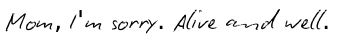
\includegraphics{OEBPS/Images/memo3.png}\\

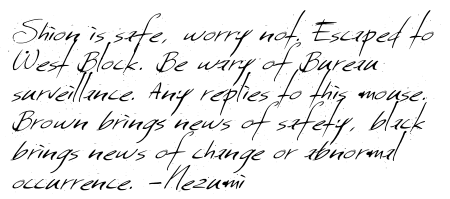
\includegraphics{OEBPS/Images/memo2a.png}\\

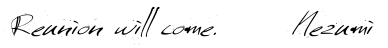
\includegraphics{OEBPS/Images/memo7.png}\\

Words could not describe how much these letters had supported
her―supported her, and kept her alive.

What will Koka turn to for support to live on? She didn't know. She
could not answer Lili's question.

"Ma'am?" Lili looked up at her. Karan nodded and flashed her a vague
smile.

I'm sorry, Lili. I've been alive for so much longer than you, and I
can't answer any of your questions.~

She heard a muffled sound in the room.

"Lili, where's Renka? Where's your mother?"

"Mommy's looking at the computer. Uncle Yoming is in there."

"Yoming?"

She held Lili's hand and walked inside. She closed the door and locked
it. The room doubled as storage, and there were sacks of flour, sugar,
and raisins piled high along with jars of honey and jam in rows.

In a far corner was Shion's bed, and beside that was an old desk.
Shion's desk. In the drawer was a half-written report that Shion was
planning to hand in.

Renka was crouched over the desk, engrossed in the monitor of the
outdated computer.

"Renka," Karan called. Renka twitched slightly and turned around. Her
bloodless face was illuminated by the dim light.

"Karan..."

"Renka, what's wrong? Has something happened?"

"Karan, it's my brother." Renka straightened up awkwardly. "Look." She
pointed at the computer screen.

Yoming was there. His fist was raised, and his expression was fierce. He
was definitely Yoming, and yet he seemed a total stranger.

"Now is our time to stand!" he declared. "If we do not stand up now to
destroy everything, we will be slaves forever! Yes, slaves! You all must
realize by now how No. 6 has deceived us all this time! How much unfair
abuse we have suffered; how much exploitation we have endured! It has
always been this way. It has always been this way, comrades. This city's
horrific history is steeped in bloodshed. Let me tell you, comrades,
about the hundreds of lives that have been banished to eternal darkness
because they disputed the authorities; because they objected; because
they resisted. Let me bring everything to light. Look, comrades!"

Yoming swept his hand towards the wall behind him.

Countless faces appeared on it. Youth, the elderly, young boys and young
girls, even infants. A girl in her wedding dress; a muscular labourer; a
thoughtful elderly gentleman; a smiling elderly lady; a sleeping infant;
a girl running this way, laughing; a middle-aged woman with her eyes
cast down; a young doctor wearing a stethoscope―many, many faces
appeared before them.

Karan's heart thudded loudly.

Da-dum. Da-dum. Da-dum.

Shion was there.

He was facing this way, with a slightly sheepish grin on his face. It
was his first birthday since coming to Lost Town, and Karan had taken a
picture.

"Aw, please, can we not take photos?"

"Why not? It's an occasion to remember."

"Fine, but no pictures outside."

"Oh, you're more bashful than I thought."

Such was the conversation that passed between them as she took the
picture.

"I want to know what kind of boy your son is. Can you tell me what he
looks like?"

Karan had shown Yoming that photo among others on his request. He had
copied the data without her even realizing.

"Look at these people," Yoming continued. "They are people who have been
taken away by the Security Bureau, never to return again. They are
people who have been murdered by No. 6. Unbeknownst to you, comrades,
the authorities have been obliterating anyone who poses an inconvenience
to them. You didn't know that, did you? No, you didn't. But I am not
blaming you, comrades. You have already come to know No. 6's true
identity. You now know what kind of people the authorities really are;
who the mayor really is. The question now is what we will do from here
on out.

Comrades, I am not talking about the past. I am talking about the
present. Even while we stand here now, fellow citizens are dying. They
are dying horrific deaths. A terrible disease is sweeping the city.
Already, many citizens―good and innocent citizens―have suffered at its
hands. But the authorities have failed to take action. Instead, they
have given themselves an effective vaccine and so are able to keep
living lives that they do not deserve.

Comrades, did you know? A considerable number of vaccines is still being
stored in the Moondrop. But the authorities are doing their best to hide
it. They won't give those vaccines to us citizens. They have paid
enormous expenses to develop them, and they don't want to hand them out
to just anyone―that's their standpoint. Have you ever heard of anything
so ridiculous?

Comrades, I disclose to you an even more shocking truth. All of this is
fact: this is something I have been investigating in secret for years.
This is the truth, and it is a horrific reality we must face. The upper
echelons of No. 6, including the mayor, have been predicting this
situation for many years―that a mysterious disease was going to spread
throughout No. 6. That was why they were developing a vaccine in secret,
while we citizens were kept in the dark. And when the situation becomes
dire, they are only interested in saving a select few. And look! Open
your eyes wide, and look at what is happening!"

Next, an image of a mob flashed across the white wall. They were people
who had crowded in protest around the Moondrop. They were all shouting
something, their expressions tense. A red ray of light streaked across
the corner of the screen. At once, every face took on an expression of
horror, and people frantically began to flee. Next, an image appeared of
soldiers at arms and several bloodied people collapsed in the square.
The video looked like it was from a hidden camera; the footage was
blurry and kept shaking sideways and diagonally.

"What is this, comrades? Do you know what this is called?"

Yoming's voice rang out, loud and pronounced.

"Yes. Our fellow people have been murdered. Killed like vermin. The
authorities have pointed their guns at their own citizens. Is that
something that ought to be forgiven? Of course not. We cannot let them
go for what they did.

Comrades, let us stand! Put the power of the government back into the
hands of the people. Take it away from the Moondrop, which has rotted
through completely. We will not stand to be trampled on anymore. We will
not be suppressed anymore. We are humans. Let us take back our freedom
and safety. To battle, to battle, to battle, comrades! We must rise up
in arms! Surround the Moondrop! Destroy No. 6! To battle, to battle, to
battle!"

It was a jarring cry. Renka turned the power off even before his yell
began to taper. Her legs curled under her as she dropped weakly to the
floor.

"It's been like this forever. About once every five minutes, my
brother's speech gets played."

Renka held her swelling belly, and her mouth twisted. The noise out on
the street grew even more agitated. It hit Karan and Renka like waves
crashing onto the shore.

To battle, to battle, to battle, to battle, to battle.

Rise up, rise up, rise up, rise up.

"Karan, what's gotten into my brother? Why is he saying things like
that? Why is he screaming?" Renka covered her face with her hands.

"Mommy." Lili huddled close to her, and placed a gentle hand on her
mother's knee. "Mommy, don't cry."

"I'm fine, Lili. I won't cry. But―but you know, Mommy is a little
scared." She then said to Karan, "My brother was such a gentle person,
but he... he looked like a completely different person... no, in fact,
he has become a different person. He's changed ever since my
sister-in-law and her baby went missing after being abducted by the
authorities... he's changed. From that day, the only thing in my
brother's heart has been―"

"Revenge."

Renka lifted her face at Karan's words, and opened her mouth slightly.
She looked like a gold fish with not enough air.

"Yoming wants revenge on No. 6. He's wants this city completely
destroyed."

"Yes," Renka answered. Her voice was croaky. "Yes, you're right, Karan.
My brother never said it. I never heard the word 'revenge' come out of
his mouth. But I knew. I'm his little sister, after all. I could tell
how he'd changed, I could tell he had vowed in his heart to get revenge.
That's why, some day... I was afraid this would happen. I was worried..
but scared. I was really scared."

Renka's lips trembled. Her large eyes turned watery, and she turned even
paler. Karan looked from Renka to the blank black screen.

Lies, she thought vehemently. I won't say all, but half of Yoming's
speech is made of lies.

Certainly, the authorities had placed its citizens under its vigilant
regime, and ruled them in a manipulative and ruthless way. It was true
that Karan and most of the citizens had been living blinded and
oblivious. Yes, many people had been sacrificed; an unidentifiable
disease was spreading like wildfire; the authorities were failing to
come up with any effective solution; they had opened fire on citizens―it
was all true.

But his claim that the city had foreseen this situation―this
unfathomable, horrific situation―and had launched the development of a
vaccine―that was false. If by some chance this was true, there was no
reason for them not to vaccinate the citizens. If they had a store of
vaccines in the Moondrop, it was unthinkable for them to withhold it.

What good did it do No. 6 to kill its own citizens? If anything, it
would do more damage than good. They were in this situation precisely
because they had no vaccine to combat the disease. Right now, they were
in the middle of a worst-case scenario.

Besides―besides―Shion is not one of them. Shion will come home. Shion
isn't someone who is "never to return again". Yoming's words were half
truth, half lies. There is no vaccine in the Moondrop. That was a lie.
He's a perfect demagogue.

Yoming was manipulating, encouraging, and agitating people's fears,
along with their long-festering suspicion and discontent towards No. 6.

Yoming, please don't. This is wrong. She thought of Koka, who had
refused to move from her son's side. She remembered her unseeing vacant
eyes, frozen open from her overwhelming grief.

The soldiers had been the ones to shoot Koka's son to death. But Yoming
was part of the cause. Yoming was deeply involved with the brutal death
of a man who had been referred to affectionately as "Good Guy Appa".

The truth was noble, as long as it remained the truth. That was how it
made the world turn. But now, Yoming was not speaking the truth. He was
twisting it conveniently to match his intentions.

"My brother has changed," Renka said in despair. "It started gradually
after my sister-in-law went missing, and when this commotion began, he
changed completely."

"You're right," Karan said resignedly.

Yoming had been waiting. He had lain low, waiting for an opportunity―not
to flourish onto the scene, but to exact revenge on No. 6.

And this was the opportune moment.

"To battle, to battle, to battle, to battle!"

His cry rumbled deep in her ears. It stirred the soul like a magnificent
soundtrack.

Karan overlapped her hands over her chest.

No, Yoming. What you're doing is wrong. What will come of involving so
many of these nameless people? What will you try to create from their
sacrifice? Can you see them? Can you see each and every person's face as
they die bleeding? Have you ever tried to look at the life each of them
has lived, and the days that they've spent?

Yoming, now is not the time to fight. We don't have a second to lose; we
have to find a way to deal with that unknown disease.

We have to protect lives, not use and dispose of them. If you loved your
wife and your son, then you should respect life all the more.

Do you―do you plan to cross that line?

Please. Cast your thoughts not to the group, the people, the citizens,
but each and every person as their own! Make a place in your heart for
me, Renka, Lili, Koka, Getsuyaku, and all the people whose names you
don't know!

You're a human, aren't you? You're not No. 6.

"Karan," Renka said in a feeble voice.

"What is it?" Karan's voice also sounded faint to her own ears.

"You know... I've wished for a long time that you and my brother would
be together."

"Why, Renka―"

"My brother liked you. I think he was in love with you. When the topic
would turn to you during dinner, he'd always turn very quiet. But he
looked so happy. I haven't seen my brother look so happy in a long
time."

"Renka..."

"Then, someday you and my brother would get married, Shion would come
home, I would give birth to my baby, and Getsuyaku and Lili would visit
you so you could get a look at the baby, too. You and my brother and
Shion would kiss the baby in turns, congratulating it, and you, Karan,
would bake a cake to celebrate. Getsuyaku and I would stretch our
savings a little to give out "Fortune Bread" to everyone in Lost Town.
They'd be little rolls that you made, Karan, and we'd hand them out as a
symbol of our happiness. We'd package them in little bags, tied with a
cute ribbon.... We'd share a little bit of happiness with everyone. Both
Lili and the baby would wear a ribbon, too. I would put a white bib on
the baby, and a light pink apron on Lili. Lili would carry a basket full
of "Fortune Bread" and we would walk down the street. Everyone would
come up to greet us, saying, 'Congratulations, Renka. Congratulations,
Getsuyaku, Lili.'"

"Renka."

"That's all I wish for. That's not greedy at all. Is it, Karan? Is it
being greedy?"

"Of course not."

It was small―such a small wish.

"Then why won't it come true? Why does everything have to fall apart and
disappear? Why?" Unable to contain herself, Renka let a sob escape her
lips. Lili embraced her mother firmly with both arms.

A small, small wish. But it could not come true.

As long as they lived in No. 6, all their hopes were like towers of
sand. They melted away all too easily. Then, what are we to do? What
must we do so we can build our lives on firm ground instead of sand?

If No. 6 isn't an idyllic city, then what is 'ideal' supposed to be? How
are we to create an entirely new world, so different from No. 6?

"Renka, Yoming isn't working alone, is he?"

"No... there must be other people who have gone through the same
thing―who have lost their family."

"And Yoming is with them, right? They must be acting together."

"Yes, I'm sure of it."

"Do you have any idea where they might be?"

After some moments of thought, Renka shook her head.

"No. It looks like they're in some basement studio. He would need proper
equipment to make that video clip."

"You're right. But neither of us know where that is. We have no way of
meeting Yoming."

"Karan," Renka held her hand out. Karan grasped it. "What will I do?
What should I do, Karan?"

Karan could feel a presence. It pressed upon her from the street.

To battle, to battle, to battle, to battle, to battle.

Destroy it, destroy it, destroy it, destroy it.

Kill, kill, kill, kill, kill.

"Let's think about it, Renka." She cupped her hand gently around Renka's
belly. Then, she touched Lili's cheek.

"We still have hope."

"What?"

"Hope. The baby in your belly, and Lili―they are our hope. We have to do
our best so that these children will have a real world to live in.
Right, Renka? We have our children. Not all our hope has been taken from
us."

"Shion, too." Renka wiped her tears away and nodded. "Shion is our hope
too, isn't he? And a big one, too."

"Mm-hmm. Thank you, Renka."

"He's coming home soon," Lili blurted without warning. "Onii-chan's
coming home soon. I can tell."

"Why, Lili." Karan scooped Lili up and kissed her on the cheek.

"It's true," she insisted. "He's really coming home."

Shion is... coming home.

Please come back, Shion. And Safu, you too.

Please come home safe.

I pray for you.

Her prayers led also to the boy named Nezumi, whom she had yet to meet.

I would love to meet you, Nezumi. I would love to see you, and thank
you. I want you to know how grateful I am for your support. Shion, Safu,
Nezumi. You, too, are my hope. My very large hope.

Come home to me.

No. 6's city hall, known informally as the Moondrop, was surrounded.

The citizens crowded the square and overflowed into the streets. Each
shouted his own words of protest. Their voices melted into one, and
boomed so loudly it seemed to shake the canopies.

But no matter how loud the clamour got, it did not reach the mayor's
office. The office was on the highest floor of the building, with
soundproof walls and windows. Whatever happened outside never disturbed
the constant silence inside.

"Why? Why has something like this happened?" The silence was broken as
the mayor spun around and shook his fist.~

"Fennec, will you calm down?" the man in the lab coat answered. "You
should be the last to be agitated." He sank deeply into the leather
chair and crossed his legs.

Pitiful, he thought as he mentally clicked his tongue. He has always
been like that. Ambitious but timid, and a coward. The man switched his
legs and recrossed them.

But he has been able to come this far precisely because he is so timid
and cowardly. He opens his heart to no one. He trusts no one. He is
suspicious of everything and acts cautiously. A fennec indeed, the
world's smallest desert-dwelling fox.

The mayor paced the room. He flitted back and forth busily. The thick
carpet absorbed almost all of the noise generated by his footsteps.

"It wasn't supposed to be this way. Citizens are supposed to gather at
the Moondrop to celebrate the Holy Day and the greatness of No. 6, are
they not? To think it would turn out like―like this, I―how could such a
thing have happened?"

The man gave a deliberate sigh. The mayor stopped pacing, and deep
creases appeared on his brow as he looked over.

"Please, Fennec," the man said. "Compose yourself. All that's been
coming out of your mouth these days is 'why' and 'such a thing'. I'm
starting to get rather bored of it."

"Answer me. Why has this happened?" The mayor's voice grew strained. The
man gave another sigh.

"Because you haven't given it your all."

"I haven't?"

"Yes. You mobilized the army, but you only cleared them away with a
handful of firearms. Surely you wouldn't call that decisive action.
Nothing is more effective than the army when it comes to subduing the
imbecilic masses. That was not the right way to use them. You should
have used them with more flourish, more decision, and an iron finality."

"You're telling me to mass-murder my citizens?"

"They'll prostrate themselves to you before they get themselves killed.
They'll bow down in awe and fear. They'll tremble as their very hearts
are seized with regret for ever opposing you or No. 6. They will be like
neutered dogs. No matter how badly they are treated, they will never be
able to bite back. Fennec, it is not too late. Mobilize the army again,
and clear away the mob that is milling in the square. It may even be
wise to use the shockwave cannon, depending on the situation and the
course of events. You've already completed on-site testing in the West
Block, have you not?"

"That's almost like―" the mayor swallowed. "That's almost like a reign
of terror."

"Reign of terror? Absurd. I have told you before: you are the ruler of
No. 6. Its King. You reign over this country. You embody justice itself
and all its forms. Opposing you is the same as defiling justice. It is
only normal to use force to make them comply."

"...Stop it," the mayor said weakly.

"Fennec, what are you afraid of? This is not like you. You have always
acted like the King that you are. You are conscious of your position as
the chosen one, and you have always lived under that notion."

"I have." The mayor slumped his shoulders, and dropped his gaze to his
feet. "I am the mayor. In No. 6's highest position of responsibility,
highest position of power. It's only natural. We were the ones that
built No. 6. We launched the revival project, and brought salvation to
the dying land and its people. We built a utopian city, the most
idyllic―most idyllic city possible by humankind."

"Precisely. You and I were both central members. In fact, only the two
of us truly understood the ideals that No. 6 strove for. The other
members were highly qualified, yes, but they lacked creativity. Or you
might say they severely lacked ambition, or an ability to observe the
changing times. But fortunately for us, we had those abilities, almost
in excess. That is why we have come this far."

"This far?" the mayor said sarcastically. "You mean being surrounded and
condemned by our citizens? Was our creativity and ambition and skill all
for this?"

"This is only a temporary situation. It will conclude instantly if only
you would take effective measures."

"Effective measures? I've taken several."

"And those are?"

"There are people fanning the flames of this chaos. I've ordered the
Security Bureau to catch them as quickly as they can."

"Any ideas as to their location?"

"Not yet. They've gone underground."

"A clearly faulty plan. You should have obliterated all such dissidents
beforehand. You ought to have destroyed them to their very roots. And
what else have you done?"

"I used all sorts of mass media to broadcast my speech. I called on the
citizens to remain calm, not to panic easily or be influenced by false
rumours. I announced a state of emergency and put a lockdown order in
effect. I commanded people to stay inside until the order was lifted,
and announced that anyone deemed as a dissident would be arrested and
detained, regardless of whether he or she is a Chronos resident. I
listened to your warning, and I... mobilized the army."

"Hm. Well, no big mistakes so far. This would have been resolved much
more quickly if you had used the army properly. But, well, small errors
can be remedied. Everything will go smoothly."

The mayor bent over and scrutinized the sitting man.

"Go smoothly? How? What part of this is going smoothly for you? The
citizens aren't retreating at all; in fact, they're out of control. No
matter how much the soldiers try to suppress them, it doesn't work. Do
you know why? Because casualty after casualty keeps occurring. Citizens
are still dying, one after another, for a reason no one can understand.
Everyone thinks that a new type of plague has suddenly broken out in the
city. They think we're hiding the vaccine somewhere. It's absurd,
absolutely absurd! That thing is no plague. It's because of them. Why
are they going around killing citizens as they please? Why? I thought
they were supposed to act however we wanted them to. I thought we had
absolute rule over them!"

The wan smile vanished from the man's face. The corner of his mouth
twitched ever so slightly.

"Fennec, how many times will you make me repeat myself? Yes, true, this
was an unexpected happening. A random, totally unpredictable event. I
acknowledge that. I acknowledge too, of course, that my predictions were
much too optimistic. But this is not as dreadful as you make it out to
be. It is nothing more than a precursor―a precursor to Its awakening."

"You're saying this chaos is just a precursor?"

"Why, yes. It is a mere response to Its awakening. Which gives you an
idea of the enormous amount of energy this thing holds. Once It awakens
completely and comes under our control, we will be able to harness that
energy, and this chaos will calm."

"Are you... really sure?"

"Have I ever lied or given you false information? I have always told the
truth. Fennec, you haven't forgotten, have you? I was the first to see
your true potential to blossom as a politician instead of a researcher."

"―I remember. You pushed for me to enter as a candidate for No. 6's
first mayor."

"Yes. You won that election, and you have reigned over No. 6 to this
day. And you will continue to. There is no need for an election. There
will be no need for the citizens to choose you of their own will.
Fennec, don't waver now. You have to act at all times like the mighty
man you are."

"A mighty man... is that what I wanted to become?"

"What did you say?" the man said sharply.

"I certainly did want to create a utopia with our very own hands," the
mayor said pensively, "and I wasn't the only one. Back then, anyone who
was involved in the building of No. 6 should have felt the same. We all
spoke about how we would realize a utopian city here, embodying the
dreams of humankind. We talked about how we would be the ones to build
its foundations. Not a single person... hoped to become an exalted man."

"A utopia cannot exist unless there is one to wield absolute power and
lead his people behind him. You should know this the best. Yes, the ones
with overwhelming power are the ones who draw the majority along with
them. If it weren't for that, No. 6 would not be called the utopia, the
Holy City that it is called today. It is a victory on the part of your
power and our ideology."

"Victory, you say."

"A complete victory," the man affirmed. "Some bumps along the way cannot
be helped. Once we overcome those, No. 6 will continue to engrave its
glorious history in time."

The mayor did not answer him. He clasped his hands behind his back, and
resumed walking.

"When will It awaken?"

"Soon."

"Soon? It isn't like you to be so vague. Be specific."

The man shrugged. Well, well. So he tells me to be specific. He must be
getting impatient. People tend to want specific numbers the more they
feel they are being cornered.

"Let me see... within twenty-four hours. All will be settled and
finished at this time tomorrow. Everything will be quiet and in its
right place."

"Twenty-four hours... I can't wait that long. Within twenty hours, at
least... no, twelve hours is the time limit."

"Impatient, are we, Fennec?"

"Impatient?" the mayor said incredulously. "How in the world could I be
otherwise in this situation? The city hall―the Moondrop―is being hemmed
in by citizens!"

The mayor's fist pounded the mahogany desk. The man shrugged one
shoulder slightly.

"Fennec, surely you don't think the Moondrop is still the heart of No.
6?

The mayor froze.

"What? What did you just say?"

"No. 6's most important function now lies in the Correctional Facility.
The Moondrop has been reduced to a mere administrative body. It can be
surrounded by anything, for that matter, and nothing serious would come
of it. As long as we have the Correctional Facility, our No. 6 is in
safe hands."

The colour receded from the mayor's face. The tip of his tongue twitched
in his half-open mouth.

"What do you mean by that?"

"Mean? I just told you. The Correctional Facility is the heart and brain
of No. 6."

"What..." the mayor croaked. His voice was overlapped by an electronic
chime. A man's long thin face appeared on the television screen embedded
in the wall. He was one of the secretaries under the mayor's direct
order.

"Mayor, there are fires happening throughout the city."

"So the rioters have found their way in to set them."

"That's one thing, but there's more. The emergency systems in all the
buildings are not functioning at all. In some buildings, I've heard that
the core computer itself has caught fire and exploded."

The man was rendered speechless. There was only the sound of his
wheezing breath whirling in his throat. What is this footage? The man
let his throat rasp even more. Some kind of trick? A scene from some
cheap drama, what? What is he showing me this for?

"The Correctional Facility is about to crumble!" The secretary's
high-pitched yell tore into him. The man, unable to endure it, took two,
three steps back.

"Wait, what's that shadow?" The mayor pushed the stumbling man back
upright again, and brought his face close to the screen.

"What is that?"

The man looked as well. It was a black shadow looming up clearly against
the flames.

"This... isn't this a wasp? No, but... wasps like this don't exist. They
simply don't." The mayor's jaw trembled.

The man's chin was also trembling. The tremor raced through his entire
body.

"Elyurias." The name slipped from his trembling lips. The mayor turned
around.

"Did you say Elyurias?"

"Yes. It is Elyurias. But, no―she is supposed to be more beautiful, more
demure. She is not supposed to be this―this enormous. She was supposed
to be controllable to my every whim."

Supposed to be. Supposed to be. Supposed to be. Supposed to be.

The screen turned black as the video was cut off.

"Mayor, the citizens have gotten inside the Moondrop. Please, be
careful!" the secretary continued to yell from the other screen.

"This cannot be!" the man and mayor's voices overlapped.

\hypertarget{index_split_002.htmlux5cux23calibre_pb_4}{}

\protect\hypertarget{index_split_003.html}{}{}

\hypertarget{index_split_003.htmlux5cux23calibre_pb_0}{}

\hypertarget{index_split_003.htmlux5cux23calibre_toc_4}{%
\subsection{CHAPTER 3}\label{index_split_003.htmlux5cux23calibre_toc_4}}

\subsubsection{This quintessence of dust}

\emph{What a piece of work is a man, how noble in reason, how infinite
in faculties, in form and moving how express and admirable, in action
how like an angel, in apprehension how like a god -- the beauty of the
world, the paragon of animals! And yet, to me, what is this quintessence
of dust? Man delights not me . . .}

\emph{-Shakespeare, Hamlet Act II Scene II~}

The doctor was much older than how Shion remembered him. The tall,
liberal man used to come to Karan's shop once or twice a week to buy a
sandwich or meat pie. A handsome beard and moustache adorned his face,
and he spoke in a beautiful, clear baritone.

He had also once invited Shion to specialize in medicine and work at his
clinic.

"You'd have no problem with picking up the necessary specialized
knowledge and technique. I recommend taking the certification exam if
you're interested."

It was an attractive offer, but Shion did not take it up. There was no
way someone like him, who had been stripped of all his privileges and
exiled from Chronos, would be able to pass the exam. But he was happy
that the doctor had looked out for him―a stranger and a mere baker's
son―and offered him a path in medicine. He was also grateful.

In the months that Shion had not seen him, the doctor had transformed so
much he hardly looked like the same person. There were white streaks in
his beard and his hair, and he looked like he had shrunk a size. But in
terms of appearance, Shion admitted he had probably undergone a more
drastic change. His hair was completely white, and his face was smeared
with blood, dirt, and soot.

The small clinic in the outskirts of Lost Town was run by the doctor, a
nurse, and a nursing robot. The nurse screamed as the bloodied, dirty
group burst in. Shion yelled over her shriek.

"Doctor, please―please, he needs treatment!"

"You... could you be―"

"The baker's son. Doctor, please. Treat him."

The doctor's eyes shifted to Nezumi. His gaze trained on the blood that
dripped from him.

"Prepare for an emergency operation."

The nurse sprang into action even before the doctor finished speaking.
She hastily disappeared into a room adjacent to the examination room. A
robot came pushing a stretcher.

"Please place the patient here."

Shion laid Nezumi down on the stretcher.

"Nezumi," he called tentatively. His eyelids remained tightly closed.
"Nezumi..."

"Please remove your arm. Please remove your arm from under the patient.
Now transporting the patient to the operating room."

The robot urged him, but Shion's arms were stiff and unyielding, still
holding Nezumi as he had all this time. Only his fingertips shook
violently.

"Shion!" Inukashi grabbed his arms and yanked them for him.

"Now transporting the patient. Now transporting the patient. Entering
emergency operating mode. Commencing oxygen intake. Commencing
measurements. Now measuring blood pressure, pulse, heart rate, blood
type."

The doctor swiftly cut Nezumi's clothes away. Several pipes grew from
the robot's torso and connected to him.

"Transporting the patient. Transporting the patient." The stretcher and
robot entered the operating room.

"Doctor." Shion grasped at the doctor's white coat. "Doctor, please...
save him. Please..."

"Shion."

He did not expect to be called by his name. Shion lifted his face.

"I'm a doctor," the man said firmly. "If someone is in need of
treatment, I will do everything in my power to give it to him. But this
is Lost Town. I don't have the equipment it takes to perform delicate
surgery."

Shion knew. But as he had told Rikiga, he had no choice but to rely on
this doctor.

"I see that he's already gotten temporary treatment. Was that you?"

"Yes."

"What kind of wound is it?"

"A gunshot. A rifle bullet pierced him."

"Pierced, you say," the doctor muttered as he strode briskly into the
operating room. Shion bowed his head deeply to the man's retreating
back.

He felt faint. He sank to the floor.

"Shion..." Inukashi sat beside him, and put an arm around his shoulders.
"Shion... I just want to ask you, do you... do you, by any chance, want
me to be with you?"

"Inukashi..."

"Listen," Inukashi said brusquely, "I've never comforted anyone before.
I used to think it wasn't worth a crumb of bread. Still think so. But...
but if you want me to comfort you right now... if I can comfort you
somehow by being here, then... then, I'll be here."

Inukashi gently rubbed Shion's arm. The tension gradually loosened, and
blood began to course through his veins again. Shion closed his eyes,
and let his head droop onto Inukashi's chest.

He felt an almost imperceptible soft bump. If this was the usual case,
he would jump up in a confused panic. But right now, he only felt
soothed. Right here, there was a body to support him, arms to hold him,
a voice to murmur to him, and the warmth of another to comfort him. This
was happiness that could not command a price. Was it not?

"Inukashi... thank you."

Oh, but... Shion bit his lip with his eyes still closed. But this is not
the warmth I long for. Not this body, these whispers, nor these arms.

Something warm flitted over his eyelids. Inukashi had licked them.
Inukashi was gently licking off the blood that had dried and caked on
them. The little mice were curled up in Shion's lap, and the dogs had
lain down in a corner of the room.

"It'll be alright," Inukashi said. "There's no way he'd die. He's not
wuss enough to give in just yet. I've seen my share of bad people in the
West Block, but no one was as cunning, conniving, and dangerous as
Nezumi. I told ya before, didn't I, that the guy is the devil himself.
You just don't know his true face. And I'm still right. He's still the
devil he always was, and devils aren't done in so easily. Tomorrow,
he'll wake up as if nothing happened, and go right back to setting traps
for us. He's that kind of guy. He'll be alright, don't worry."

Shion opened his eyes, and lifted himself up.

"Inukashi, I'm grateful. Thank you so much."

"I was only insulting Nezumi, dumbass. What're you feeling grateful
about? You're a hopeless idiot, you know. Hopeless."

Inukashi turned aside obstinately. But he did not move away from Shion.

Ungh, nghoaaaar, nghoaaar.

A snore rang out, making the very air of the room vibrate.

"Whoa! Will ya listen to that racket."

Nghoaaaar, nghoaaaar, nghoaaaar, ungh, ungh.

Rikiga was fast asleep, lying on his back on a bench.

"Just now he was saying he wouldn't be able to sleep without some drinks
in him, and now look at the guy. Like a log. I'm surrounded by hopeless
people." Inukashi sighed theatrically. Then, he gave a short whistle.
The dogs got to their feet and approached. They nestled close to
Inukashi and Shion, and lay crouched on their bellies.

"These guys can make the best sleeping quarters out of any hole. It's
time for us to catch a wink, too."

"Yeah..."

"We need to sleep, Shion." Inukashi pulled at Shion's shirt. "We won't
be able to fight tomorrow if we don't. You don't think our fight is over
yet, do you?"

He did not. Nothing had been solved yet. The fight would still continue
tomorrow. But if I lost Nezumi, if I had to face a tomorrow without him,
then I wouldn't be able to remain a soldier.

You're weak. Unbelievably frail, he could hear Nezumi say in derision.
Laugh at me, Nezumi. Look on me with contempt. Make fun of me. Give me a
scornful laugh, a cold laugh. I just want to hear your laughter. Let me
hear it, please.

"Sleep," Inukashi said, almost like an order.

The Correctional Facility was burning. The flames roared up around it as
it crumbled. This is a dream, his reason told him. You've escaped the
Correctional Facility. You're already in Lost Town, No. 6. That's
why―this must be a dream.

This is an illusion.

The flames roared. They were revoltingly real. He could clearly see the
tip of each writhing flame. His skin smarted at the scorching air that
blew at him. The acrid smell stung his nose.

This is a dream? This is an illusion? Absurd. This is unmistakably
reality.

But does that mean I've come back again? Have I slipped back in time to
right after I escaped the Correctional Facility?

The flames burned with even greater vigour. They roared, wavered, and
overlapped. He saw them stretch out into thin strips before a black
streak slashed through it.

Shion stood stock-still with his breath held. All confusion, agitation,
and astonishment fell away. He simply stood in a trance.

The black streak kept widening. The flames split into two.

"A wasp..."

The rest failed to materialize as words.

It had a coal-black body, a slender curved torso, a long belly,
transparent wings embroidered with thin golden lines; golden antennae
and compound eyes; three simple eyes that shone a dull silver.

A giant wasp appeared out of the flames. It was a wasp, coloured
coal-black, gold, and silver―light and darkness. Shion took a step
backwards. Its beauty was almost terrifying. He was so overwhelmed, he
was almost brought to his knees.

What... is this?

"Elyurias," a mutter touched his earlobe.

"Nezumi."

Nezumi was standing right beside Shion. He stared unblinking at the
flames. No―he was not looking at the flames engulfing the Correctional
Facility, but at the enormous wasp. Nezumi was holding his ground
against it.

"Elyurias? This wasp?"

Nezumi did not answer. He did not stir. He was almost like a statue. For
an instant, the wasp in front of Shion faded in his consciousness.
Nezumi was standing there. His eyes were open wide. His profile
expressionless, but blood coursed through that face.

"Nezumi, you really did―" You really survived.

Nezumi inhaled. His lips moved very slightly. A melody flowed forth.
Gentle music found life as it left Nezumi's lips.

Shion smelled the lush scent of greenery. The sound of the rustling
canopies reached his ears. He felt the beating of wings. The buzzing of
small insects echoed in his eardrums, until even that melted into music,
forming its ebb and flow.

His body was being lifted up. He no longer knew where he was. His body
and soul were suspended in Nezumi's music. Shion let his whole body
relax as he lent himself fully to it.

He could hear singing.

The wind steals the soul away, humans thieve the heart

O earth, wind, and rain; O heavens, O light

Keep everything here

Keep everything here, and

Live in this place

O soul, my heart, O love, my feelings true

Return home here

And stay

The wind steals the soul away, humans thieve the heart

But here I will stay

to keep singing

Please

Deliver my song

Please

Accept my song

Shion had broken into a thin sheen of sweat in the midst of his ecstasy.
A bead of sweat slid down his forehead.

Suddenly, he was blasted by hot air.

He was slammed to the ground. Charred pieces of debris grazed his
cheeks, his body, as they bounced and tumbled across the ground.

"Don't get up." Nezumi's hand pressed on his back. "Keep lying low."

The wind kept blowing. Fragments of rock and debris rolled over the
ground in front of Shion as he lay face-down on the ground.

Chuckle chuckle chuckle.

Chuckle chuckle chuckle.

Laughter welled up from deep underground. Or was it raining down from
the heavens?

Chuckle chuckle chuckle.

Chuckle chuckle chuckle.

The wasp spread its wings wide open. The flames streamed sideways,
crawling across the ground.

Chuckle chuckle chuckle.

Chuckle chuckle chuckle.

The wasp took flight. It ascended to the sky without a sound, leaving
only the wind behind. A piercing buzz of wings rose all around.
Thousands of small black specks took flight after the giant wasp. The
swarm of them formed a wide band as they rose.

"Elyurias," Nezumi murmured again.

He couldn't breath. There was something weighing down on his upper
torso.

Shion awoke. Inukashi's head was on his chest. He was asleep with his
ear pressed to Shion's chest as if to check his heartbeat. He was
breathing softly. Two dogs were nestled close on either side of them.

I see what he meant. You definitely wouldn't freeze to death like this.

Another dog was curled up beside Rikiga. Despite his grumbling, Inukashi
had also looked out for Rikiga to make sure he didn't freeze. Perhaps
that explained why Rikiga's snores had turned into peaceful breathing.

They were in a small hospital room, Lost Town, No. 6. There was no
mistake: time had not turned back. But that was not a dream. What he had
seen was reality.

Elyurias―was that it? A wasp born from a cocoon of flames?

Shion gingerly touched the nape of his neck. He thought about the wasp
that had tried to tear through that spot and crawl out of it. He thought
about Yamase. He thought about the thousands of wasps which had taken
flight in a dense black stream. If those were all parasitic, what would
become of No. 6?

He did not know.

He slipped a couch cushion under Inukashi's head, and stood up
stealthily so as not to wake him. He had probably only been asleep for a
short while―not more than thirty minutes. But his body felt surprisingly
light. Was it because he was relieved?

Nezumi survived. He was certain. His heart, which was fraught with
tension until then, gradually began to unwind. Shion took several deep
breaths.

He was concerned about where the wasps were going, as well as what kind
of fate awaited No. 6. But his relief at not losing Nezumi trumped it
all.

He inhaled once more, deeply, and exhaled.

A computer was embedded in the doctor's desk. He pressed a button, and
the screen silently began to load. He dug into the pocket of his
sweater.

"There it is." The chip had been given to him by the man called Rou. He
wondered what was going to happen to that underground area now that the
Correctional Facility had crumbled. What had happened to Sasori? Or the
boy who had handed him a bowl of water? The girl who had stared at Shion
in wonder? And Safu?

Rou had said that the chip contained the entirety of his research, and
that he entrusted it to Shion.

"After you have saved your friend, please try to decode it." His voice
had been hoarse and feeble. After you have saved your friend...

Safu. I couldn't save her. She had been his precious friend, and he had
abandoned her.

His last glimpse of Safu had been of her smiling. She looked a little
more mature than Shion remembered, and she was beautiful.

I couldn't save her. In the end, I couldn't save her.

He made a fist and struck his chest. I've made another wound here. A
wound that'll ache for the rest of my life. I'll never forget. I won't
be able to forget.

Safu. You're forever out of reach, no matter how strongly I feel for
you. But you'll still be in my heart. I'll continue to think of you, and
of what you left behind for me.

He inserted the chip. He was not asked for a password. Shion bent
forward and stared intently at the screen.

Everything to do with No. 6 during their underground conversation with
Rou was written here. Elyurias, the Mao Massacre, the Forest People,
destruction, predation and parasitism....

As he read on, wading through the mix of unintelligible technical
language and numbers, he felt his fingertips growing colder.

Shion finished reading, and extracted the chip. His mind was half-numb
and in a daze.

So this was No. 6.

This was Elyurias.

The door of the operating room opened and the doctor walked out.

"Doctor." Shion stood up, and the man nodded at him.

"He'll be alright. He's hanging in there."

"Thank you so much, doctor. Thank you."

The doctor removed his mask and grinned.

"You mentioned that you were the one who stemmed his bleeding and gave
him temporary treatment?"

"Yes."

"You did a very nice job. He was also lucky that the bullet hadn't
remained in his body. It pierced him, but thankfully it just missed the
fatal spot. He's very fortunate, indeed."

"I told ya so."

Shion had not noticed Inukashi standing behind him. Inukashi had a hand
on his hip, and shot a quick glance at Shion.

"Nezumi has a notorious amount of good luck when it comes to getting out
of bad situations. You don't need to worry about him."

"And I think I need to worry about the rest of you," the doctor smiled
crookedly. "Where were you hit, Shion?"

"You know my name?"

"I do. It did make the headlines when you got arrested and taken to the
Correctional Facility."

"I see..."

"Everyone who had any knowledge of you was surprised. I don't think
anyone could believe that you were the 'fallen elite turned murdering
monster' or the workplace murder suspect that the authorities made you
out to be."

"You too, doctor?"

"You could say that. I was more pained than surprised. I'd caught on
that the authorities were trying to paint a false picture of you as a
criminal."

The doctor then let out a long breath.

"It was the same with my younger brother," he said.

"Your brother?"

"Yes. We were far apart in age. Our father passed away early on, so I
raised him like a son. He was abducted by the Security Bureau five years
ago, when he was eighteen. Take a guess at why."

"Because he refused to declare his loyalty to No. 6?"

"Absolutely right. My brother refused to partake in the allegiance
ritual held at their school every morning. He didn't like being forced
to submit. I think it came from his youthful pride and sense of justice.
And as a human, it was normal for him to feel this way. My brother was
indeed a proper, normal adolescent. Maybe he was a little more
rebellious and stubborn than most. He was also a little inexperienced in
the ways of the world. My brother was summoned to the Moondrop the same
day, and he didn't come back until two weeks later."

"He came back?"

"He came back, but he was transformed. I don't mean dead―he was alive.
But he may as well have been dead. You could see no remnant of the
cheerful, active captain of the basketball team that he used to be. He
hardly spoke or responded to me, and just gazed blankly at the sky all
day, just vacantly stared.... He killed himself not long after coming
home. I can't even bear to think about what he must have gone through
during those two weeks. I said he killed himself, but in truth, he was
murdered by this city. Our mother collapsed from shock, and she never...
she passed away not more than three days later. Her will to live was
torn from her once she saw what her beloved son was reduced to. Our
mother may as well have been murdered, too. No, she I believe was. It
was definitely murder." The doctor nodded vehemently as if to convince
himself.

He killed himself.

Shion recalled the doctor's words in his head again.

In the idyllic city of No. 6, cases of suicide were infinitely close to
zero. All citizens were promised blissful and peaceful lives. But what
an empty, artificial promise it was.

The doctor bit his lip as if to endure a throbbing pain. This man had
also suffered at the hands of No. 6. Already how many lives had the city
devoured?

Shion clenched his hand into a tight fist.

No. 6 did not permit people to be people, nor for each to be his own.

Why? he almost screamed. Rou said so. He said he tried to construct a
utopia―one without war, discrimination, or unhappiness.

When did it go wrong? What went wrong to transform it into such a
ruthless monster? What went wrong―?

The doctor's face unravelled into a smile as his lips relaxed.

"But Karan was fearless. She continued to open her shop, bake bread, and
put it on the shelves. Every time I passed Karan's bakery, I couldn't
help but breathe in the delicious aroma of freshly-baked bread. She is
amazing for carrying on her daily work in spite of her loss. She
probably strongly believed that you were going to come home. I felt pity
for Karan, you know. I thought there was a slim chance, if there was
even one, that you were coming home. I believed if you did come back,
you would be just like my brother. But you did come back, and in one
piece. You came back proper."

"I did change in appearance, though."

"Appearances don't matter, as long as your soul isn't broken. That's
precisely No. 6's plan―to govern human souls. To rule the hearts, minds,
and even thoughts of people."

Inukashi stifled a huge yawn.

"So tell me what else is new. I thought this was obvious to you guys
already. For us West Block residents, No. 6 ain't no utopia. It's like a
bloated, fat vampire."

"A vampire... I can see that." A smile spread across the doctor's face.
"And that vampire is writhing in pain from the changes occurring in its
body. To think―to think this day has come―ha ha ha! I wish I could have
shown this to my brother and mother! Ha ha ha ha!"

The doctor's laughter gradually gained momentum until it became a roar.
Inukashi furrowed his brow and recoiled.

"Hey, Shion. Is the doc okay? I mean, up here?" He pointed at his head.
"You sure he hasn't got something loose in there?"

"He saved Nezumi's life," Shion said sternly.

"Sure didn't do anything for me," retorted Inukashi.

The doctor was still laughing. Shion slowly enunciated his words as he
spoke at the man's trembling back.

"Doctor, can I see Nezumi?"

The laughter stopped. The doctor turned around. The echoes of his
laughter and the residue of his mirth still swam in his eyes.

"Nezumi? Ah, you mean that boy. What a peculiar name. Not his real name,
is it?"

"I don't think so."

"And what is?"

He had opened his mouth to say "I don't know" when the door to the
examination room opened a crack. A tall, thin man was edging his upper
body into view. A crow was perched on his shoulder. The mice gave a
terrified screech. One dove into Shion's pocket, while the other two
squeezed under the belly of a dog with patched fur.

"Yoming, what's the matter?" The doctor strode over to the man. Yoming
whispered something into his ear. The doctor's eyebrows rose
dramatically.

"The Correctional Facility!" The doctor's mouth gaped open. "The
Correctional Facility―is that even possible?"

Yoming answered him. Shion could not catch it. He didn't want to. Right
now, he was in no mood to listen.

I want to see Nezumi. All of his thoughts concentrated into that one
point. His heart pounded in anticipation.

I want see him and know that he's alive.

Shion put his hand on the operating room door.

"He's upstairs." The doctor pointed an index finger straight up at the
ceiling. "There's a recovery room on the second floor. Aria is attending
to him. There's a direct-route elevator in the operating room, too, but
I want you to use the stairs in the hallway."

"Thank you, doctor."

"Oh―wait a minute," the doctor said. "Don't tell me you've come from the
Correctional Facility―"

Shion did not hear the last of the doctor's sentence. He tore into the
hallway.

"Hey, wake up, old man! Looks like we're paying Nezumi a visit. We need
to get some flowers."

"Nnngh, what? Who said I ever wanted to go?"

"Quit talking in your sleep and wake the hell up."

Shion left Inukashi and Rikiga bickering behind him, and dashed up the
stairs. His legs faltered for a moment as he reached the corridor, dimly
lit by nighttime lights.

It reminded him of the long, straight corridor of the Correctional
Facility. But this atmosphere was not impregnated with fear; it did not
prick his skin as before.

He exhaled softly.

Only one room by the stairs had the lights on. Shion regulated his
breathing, and gently placed his hand on the door. It slid silently
open.

The room walls were painted a pale yellow. Across from him, darker
yellow curtains were drawn across what he supposed was a large window.

By the window, the nursing robot was making faint electronic sounds by
the bed. When Shion entered, it raised its arm as if to reject him.

"Resting. Resting. Not taking visitors. The patient is resting. Not
taking visitors."

I see, this robot must be Aria. He bent low to talk to the robot.

"Aria, thank you. I'm very grateful."

"Grateful. Grateful. Grateful." The nursing robot's visual sensors
flashed, and turned from red to green. It seemed to have acknowledged
Shion's presence.

"Aria, I want you to let me see your patient. I want to see him really
badly. I'll do anything."

Aria's visual sensors stopped flashing―or rather, she stopped blinking.
Her green eyes were fixed on Shion.

"Want to see. Want to see. Request accepted. Request accepted."

Aria glided across the floor. She retracted her arm, and settled herself
in a corner of the room. She looked like a quirky but lovable piece of
interior decor. The dogs lay around her peacefully.

Nezumi was sleeping on the bed. He was connected to many tubes, and his
eyes were closed. A tinge of colour had returned to his cheeks, perhaps
thanks to a blood transfusion. His superfibre cloth was folded neatly
and placed beside the bed, no doubt by Aria.

Shion bent over Nezumi and took his pulse. It was faint, but regular.
Shion could definitely feel it. A sigh of relief escaped his lips.

"Nezumi..." He felt his body unravel as he released a sigh.

He made it. He survived. Shion knelt by the bed and buried his face in
the sheets. He could feel Nezumi's heartbeat. He wanted to raise his
voice and cry―as loudly as his voice would allow.

He's alive. He's alive. Nezumi's alive.

"I could do with a few more winks." Rikiga yawned, showing a full array
of teeth.

"I'm hungry," Inukashi said. "And my dogs are hungry, too. It's all good
that Nezumi made it, but it ain't gonna be funny if we die from
starvation instead. Ah damnit, I'm starved!"

"If 'we' die? Don't lump me in with the likes of you."

"You've got nothing to do with it, old man. I'm talking about me and my
dogs. Hey, robot, uh―Aria, was it? Struck lucky with a pretty name,
haven't ya? Doesn't suit you at all. So, Ms. Aria, can you get us some
grub or what?"

"Grub. Grub. Grub. Cannot comprehend. Cannot comprehend."

"I mean a meal. Patients and injured people still need to eat, right?"
Inukashi made a motion of wolfing something down.

"Meal. Understood. Understood."

Aria's torso opened up. A row of three steaming paper cups appeared.
Inukashi whistled, and Rikiga swallowed hungrily.

"Two more, two more," Inukashi said."For my dogs. And some bread and
meat, if you've got any."

"No meat. Have bread." Her torso opened again. Two more paper cups and
some rolls appeared.

"You're the best. I think I might fall in love with you. I'd give you a
huge kiss."

"I wouldn't do that," Rikiga said. "Think of the poor robot who has to
get a kiss from you. It would probably stop functioning. Don't turn such
a good girl into a lump of scrap metal. Hm? What's this?"

Rikiga furrowed his brow as he brought the cup away from his lips.

"It's bland. It may as well be hot water. And this bread... it doesn't
taste like anything."

"It's hospital food, don't complain about it. Look how easy it was to
get hot soup and bread. Can't beat No. 6. In the West Block, you could
only dream of a feast like this. Right, Shion?"

"Yeah. It's really tasty." He was not simply going along with Inukashi.
He really found it delicious.

This taste almost matched that of the rich soup that Nezumi made on the
day he had escaped to the West Block―the day he had miraculously lived
through the wasp's attack.

It soaked into his body, quenched his soul, and revived him. Just one
cup of soup restored his confidence that he would live through another
day.

It's delicious.

Nezumi, wake up. Wake up so you can sip this cup of soup. Look at me
again with those eyes full of life.

"Mm..." Nezumi shifted. The whiteness of the bandage around his shoulder
and chest stung Shion's eyes.

"Nezumi, Nezumi!" Shion called to him. He poured his soul into the name
he had called so many times before. Nezumi's eyelashes fluttered ever so
slightly.

"He's probably still knocked out from the anaesthesia," Rikiga said. "He
won't be waking up for a while. Hmm, but even a devil like him looks
like an angel when he's all quiet and asleep like this. Strange, isn't
it?" he murmured pensively.

"Hah, you still hung up on him, old man? How many times have you been
shafted because you were fooled by his looks?"

"I've been shafted enough times, with or without his good looks. By both
Eve and you." Rikiga sighed. "Am I just going to spend the rest of my
life being bossed around by rude, filthy brats? Just thinking about it
makes me depressed. I need a drink to stomach this. Lady Aria, you don't
happen to have some booze on you, do you?"

"Booze. Booze. Booze. Cannot comprehend. Unable to process your
request."

"Alcohol. You know, I want something that'll hit me in the guts with
some oomph."

"We have: alcohol antiseptic. We have: disinfectant alcohol. We have:
sterilization alcohol. Which one do you need? Which one do you need?"

"I don't need any of that. I don't need antisepsis, nor do I need to be
disinfected or sterilized. God, what a useless princess." Rikiga clicked
his tongue.

Inukashi turned aside and laughed discreetly. Shion also couldn't help
but twitch the corners of his mouth. Rikiga wore a wry smile. The three
glanced at each other and laughed for some time.

"I never expected you'd make it back like this," Inukashi murmured
thoughtfully after their laughter had died down.

"Me neither," Shion agreed.

"Not to mention that bonus work you guys did with the Correctional
Facility. I have a bit of a new regard for you, to tell you the truth. I
honestly never expected―had no clue how you'd pull it off. I thought you
guys would never be able to escape through the garbage chute."

"It's thanks to you and Rikiga-san, Inukashi."

"Thanks to us, huh. Say, Shion..."

"Hm?"

"Didn't it ever cross your mind that we might not show up at the waste
depot? What if we pulled a no-show, or we showed up but left early―you
didn't think about that at all?"

Shion searched his soul for a moment at Inukashi's question. What had he
thought back then? He searched, then gave an answer.

"I didn't think of it at all." He gazed into Inukashi's eyes. "That
never even crossed my mind. I believed that you and Rikiga-san would be
there. Nezumi must have thought so, too. I'm sure he had solid belief in
you."

"Well, that's all great and nice for you, but let me say that we...
well, I dunno about the old man, but... I don't owe nothing to you guys.
I didn't have an obligation to wait in there."

"Me neither," Rikiga chimed in. "I might have my share of grudges, but I
don't have any obligation or debts to owe, either." He clucked his
tongue repeatedly.

"Lemme tell you something, Shion," Inukashi stabbed a sharp-clawed index
finger in Shion's direction. "Don't think I got myself involved in this
hell of a mess for free. You guys owe me now. You best be prepared,
'cause I'm putting hefty interest on it."

"I'll have you know that I'm going to be sending out an invoice
addressed to Eve as well. He's made me spend quite a bit of money,
taking everything into account. I wouldn't be able to rest in peace if I
didn't get reimbursed for that at least."

Inukashi and Rikiga grimaced at the same time as if they had rehearsed
it. Shion suppressed a laugh and nodded solemnly. He didn't care how
astronomical the interest rate was, or how exorbitant the invoice was.
The two had stayed and waited for them. In that hygiene management room,
where life and death jostled each other, they had continued to wait,
believing that Shion and Nezumi would return alive.

He bit his lip.

Safu had also been waiting. She had been waiting for Shion. She was
probably waiting for him, not to say goodbye, but to escape together
with him.

I couldn't hold up my end.

He had not been able to give her what Rikiga and Inukashi had given him.

"Hey, Shion." Inukashi hugged his knees and leaned closer. "Whaddaya
think is gonna happen to the West Block?"

"The West Block, huh..."

"Yeah. No. 6 is spiralling into chaos, by the looks of it. The
Correctional Facility is gone. The gates are blown apart. Maybe that
wall―the wall that separates the West Block and No. 6―maybe that'll
break down too. Ya think?"

"Yeah. In fact, it most likely will."

Inukashi swallowed, and curled up just slightly.

"So, if that happens, I wonder what everyone in the West Block is gonna
do. How would they face people who've treated them like crap all this
time? Would they take their anger out on them? Would they storm into No.
6? Would they fight, or run away... wonder what they'll do? When I think
about it, I just... well, it makes my head spin."

"Mm-hmm..." Inukashi was right. It made his head spin, too. A world
without walls: it was beyond his imagination. What would hold ground
there? Surely not just peace and open freedom. How would the West
Block's wind, swirling with hatred and anguish, blow against No. 6?

It simply exceeded his imagination.

"Turn the lights out," said a low, cutting voice.

"Wh―Eve, are you―?" Rikiga fell speechless.

Nezumi was sitting upright. His dark grey eyes glinted sharply. "Turn
off the lights. Quickly," he repeated.

Inukashi's nose twitched. He jumped to his feet, and pressed the
electric switch. All the lights were cut, and darkness fell over Shion's
vision like a veil.

"Nezumi, what―"

"Shh!"

Nezumi moved in the darkness. He pulled out all the tubes that were
inserted into his arm. He slipped to the floor and knelt down.

"Keep quiet. Don't even move."

Inukashi shivered.

Time passed. One minute, two minutes, three minutes... suddenly, noise
erupted from downstairs. Footsteps, shouting, screaming, then gunshots.

"Run! It's the Security Bureau!"

"Don't move. Move, and we will shoot."

"Run! Get out of here!"

"All you traitors are under arrest."

"Kill them, it's no big matter."

"Their leader is getting away! Get him, and kill him!"

Those were the few words that Shion's ears managed to catch.

He curled up in the darkness.

He curled up and sat still, feeling Nezumi's warmth and breathing right
beside him.

\hypertarget{index_split_003.htmlux5cux23calibre_pb_6}{}

\protect\hypertarget{index_split_004.html}{}{}

\hypertarget{index_split_004.htmlux5cux23calibre_pb_0}{}

\hypertarget{index_split_004.htmlux5cux23calibre_toc_5}{%
\subsection{CHAPTER 4}\label{index_split_004.htmlux5cux23calibre_toc_5}}

\subsubsection{Out, out, brief candle}

\emph{Tomorrow, and tomorrow, and tomorrow}

\emph{Creeps in this petty pace from day to day,}

\emph{To the last syllable of recorded time,}

\emph{And all our yesterdays have lighted fools}

\emph{The way to dusty death. Out, out, brief candle.}

\emph{Life's but a walking shadow, a poor player}

\emph{That struts and frets his hour upon the stage . . .}

\emph{-Shakespeare, Macbeth Act V Scene V}

Just once, he heard footsteps approach. Someone was trying to run up the
stairs. But the footsteps died along with a gunshot, a scream, and
someone tumbling down the stairs. He didn't have to see it to know what
happened. The same stairs that Shion had flown up moments ago was
probably spattered with someone's blood.

Not only the stairs. The floor, the entrance, and the consultation room
were probably smeared with blood and littered with broken objects in a
horrific scene. A body or two probably lay on the floor.

What about the doctor? What had become of the man who saved Nezumi's
life?

"Don't move." Nezumi restrained his arm. "Don't move yet."

Shion, Inukashi, and Rikiga all held their breaths and tensed as if they
were bound by his words. Even the dogs lay low to the floor, unmoving
like boulders, save to growl softly at the footsteps.

One minute, two minutes, three minutes....

"Freedom for No. 6! Freedom for all of us!" A hoarse, high-pitched
scream resounded, its gender indiscernible. Right afterwards, angry
voices and the sound of fierce beatings were heard through the window.

It's the same. Shion made a fist. His palm was damp with perspiration.

It was the same―no different from the Hunt in the West Block. The
brutality he had seen under the thick snow clouds was taking place again
right here.

Stealthily within the walls, openly outside of them―that was the only
difference.

The sweat stung the countless cuts on his palm and made it throb
slightly. Sweat streamed down his cheek, and entered his mouth.

In No. 6, he used to feel trapped and suffocated, like being forced to
wear clothes that didn't quite fit. But until Nezumi had saved him and
they had begun to live in the West Block, he had never had much
difficulty dealing with these vague doubts and feelings of suffocation.
Not until he was given a chance to look at No. 6 from the outside. In
fact, he had taken comfort in No. 6's cleanliness and abundant
lifestyle. It was true. He had been devouring this comfort and taking it
for granted. Back then, the Security Bureau's existence hardly crossed
his mind. It never had to; the days still went by. On the surface, time
passed peacefully without incidence.

When had it all begun?

Shion was wheeling his bike across the park after his shift. He was
allowed to ride his bicycle in the park, as long as he didn't go over
the speed limit. But the spring sunset was so beautiful that Shion had
felt like taking a stroll to take it all in.

The sky was divided into dark pink, red, and carmine. The streaming
clouds caught the sun, their edges glittering golden. The sweet
fragrance of the flowers blended with the refreshing scent of new
leaves, enveloping the passersby.

"Ah, the end of another day."

"It was wonderful, wasn't it?"

"All's right with the world, as they say. What do you say to topping it
all off with a mouthwatering meal and some excellent wine?"

"Oh, how splendid. That sounds great."

He could hear the lighthearted conversation of a young man and
woman―were they lovers, husband and wife, or good friends?

They're right. It's a perfect evening to enjoy wine over a nice meal in
the company of someone close, Shion had thought, feeling a comfortable
sort of weariness and hunger himself.

All's right with the world.

Neither Shion nor that man or woman had any clue about what lurked in
the depths of that day. Most people didn't. It wasn't because of the
dreamy spring evening. Through hot summer days, sleety mornings, in
autumn sunsets, they had never noticed.

The majority of the citizens were neither concerned nor interested about
the Security Bureau. They probably had no idea that it would bare its
fangs so ferociously at the slightest voice of protest from the
citizens. They thought of the Security Bureau as an organization that
maintained and protected their safety―an organization for the
people―were they not? And they believed in this clause―

No. 6 exists for its citizens. It exists to ensure a plentiful and
comfortable life for its citizens. No one shall be permitted to threaten
the safety, activities, and lives of the citizens in any way whatsoever.

They believed the city would also abide by this clause of its own City
Charter. The people relied upon the city, left everything in its hands,
and unwittingly allowed themselves to be pulled along by its flow.

And this was the result.

The sweat stung in his wounds. Nezumi's hand was still restraining
Shion's arm.

If this was the result, then Nezumi―where did we go wrong? Do you know
the answer?

No―I'm the one that needs to know the answer, not you. I was born as a
No. 6 citizen, reaped all of its benefits, and lived without any concern
for the outside or inside. I'm the one who has to reach out and grasp
the answer, in exchange for always choosing the comfort of lending
myself to the least resistant path, rather than struggling against the
current.

I know. Meeting you has taught me, and so have the words we exchanged
and the days we spent together. I need an answer that I've grasped with
my own hands, rather than one that's been prepared for me.

Mine, and not someone else's.

Or else I'll end up with the same result again.

"They weren't after us, then." Shion sensed Inukashi twitching his nose
in the dark. "I was totally under the impression that... the doctor
tipped the Bureau off. Looks like that wasn't it."

"No, it definitely wasn't."

Traitors. That was what the Bureau officials had said. The target of
their sting had not been Shion, but the others―the doctor, and Yoming.

Inukashi twitched his nose again. "Nezumi... aren't we safe now?"

"Wait. It's still too early."

"Tsk, paranoid as always."

One minute, two minutes, three minutes....

"Hey, Nezumi."

"Don't rush. But―alright, it should be fine now. Don't turn on the
lights. Leave them off, and move quietly."

Nezumi pushed the door slightly ajar, and whistled softly. Hamlet poked
his head out from Shion's pocket, alighted on the floor, and dashed
through the open crack.

Momentarily, a lighthearted squeak greeted them.

Cheep cheep, chit-chit-chit.

Cheep cheep, chit-chit-chit.

"Alright, let's go downstairs. Avoid the elevator, just in case." Nezumi
swiftly wrapped the superfibre cloth around himself, and slipped into
the hallway.

"What the hell was that?" Shion saw Rikiga's mouth gaping open by the
light that spilled in from the hallway. "Wasn't he unconscious just now?
Or was that an act, too? Playing the part of a prince on his deathbed?"

Inukashi shrugged.

"He ain't no prince. He's an animal. Like a savage beast. No way he can
sleep in the face of oncoming danger. He sensed the Security Bureau guys
before my nose could sniff them out, damnit. Pisses me off."

"I see. Now I have a good idea of how Eve could have survived this far.
With instincts as sharp as those, and that cautiousness to boot..."

"Falling in love all over again, old man?"

"I just confirmed my notion that he doesn't have an ounce of good in
him."

The humans, dogs, and mice crept down the stairs cautiously, step by
step. There was a pool of blood in the stairwell. At the bottom of the
stairs was the owner of that blood, a man in his forties or fifties
lying on his back.

The lower floor was just as grisly as Shion imagined. Blood had sprayed
the walls and the floor. There was broken glass and furniture strewn
about, all soiled with dirt and blood. At the end of the hall, a
blue-grey door was half-open. The room was dark and the air inside
cold―a basement room, perhaps.

A man lay slumped against the door, and the nurse at his feet. A figure
clad in a lab coat lay a few metres away. The three of them were
perfectly still.

"Doctor!" Shion ran to him and lifted him up in his arms. The chest of
the man's lab coat was dyed in blood. "Doctor, answer me, please."

His words felt painfully empty as they escaped his lips.

The doctor was clearly almost dead. There was no hope for him.

"Doctor, doctor! Open your eyes, please," Shion continued to implore
with empty words. That was all he could do.

The door to the consulting room opened, and Aria appeared, evidently
from the elevator.

"Vital signs: none. Vital signs: none. Vital signs―minimal. Minimal."

The doctor's eyelids slowly lifted.

"Vital signs: minimal. Commencing treatment."

Several tubes extended from Aria's torso, and connected to the doctor's
body.

"Aria... don't. It's no use..."

"No use. No use... cannot comprehend. Continuing treatment."

"Doctor, what... why did this happen?"

"...He... broadcasting... from the basement of this clinic... calling...
on his comrades to defeat No. 6 together..."

"Vital signs: minimal. Probability of recovery: one percent. One
percent."

"I wanted revenge... on No. 6... revenge..."

"Doctor," Shion pleaded.

"I wanted to... destroy this world... and build it... anew."

Suddenly the doctor dug his fingers into Shion's arm.

"Shion," the man called his name in a clear, strong voice. "I leave this
in your hands."

His eyes were open wide, fixed intently on Shion.

"I leave it... in your hands. Don't ever make... No. 6... this kind of
city... again. Please. I'm leaving it to you."

The doctor's fingers slipped out of his own. The light went out of his
eyes as they glazed over. His whole body convulsed.

Then, it was over.

"Vital signs: minimal. Minimal. Unable to register. Unable to register.
Aborting treatment."

"Doctor..."

Shion laid the man down, and put a hand over his eyelids. With his eyes
closed, the doctor looked peaceful and relaxed.

"Leave it to you, huh." Inukashi let out a long sigh. "You guys are the
ones who built No. 6 in the first place," he said to the doctor's body.
"But once something goes wrong and it spins out of control, you just
shove it off onto someone else? Not exactly a friendly gift to leave to
someone, is it? A little selfish, don't you think, doctor? I guess it's
none of my business, though."

"Inukashi, what good is it to mouth off at a dead man? He's not going to
hear any of it. Poor guy." Rikiga clasped his hands in front of his
chest and bowed his head.

"The hell are you doing?" Inukashi asked.

"I'm praying to God, can't you tell? O God, please forgive this sinful
man. May you bless his soul and let him rest in peace by your side."

"Hah, you don't even believe in God. What an act. Oh, wait―you must be
praying to God Moneybags Almighty, right, old man?"

"Rotten kid," spat Rikiga. "You never get tired of spewing insults, do
you? Once this settles down, you're in for it. You remember that."
Rikiga unclasped his hands and rolled his shoulder joints.

"So, what now?" he said. "We've accomplished our big goal of destroying
the Correctional Facility. As for me, I'm in the mood for heading back
to the West Block and crawling into bed. I feel like curling up and
dreaming about digging up gold from underneath the Correctional
Facility. I'd wake up to the best morning ever. It puts me in a good
mood already."

"Old man, you can be sarcastic all you want, but Nezumi's not gonna
respond. I'd get a better response out of complaining to that corpse
over there." Inukashi chuckled spiritedly, his shoulders shaking with
his laughter.

"But truth be told, I'm all for crawling into bed myself. And, well,
there are a lot of things that I want to mull over. It doesn't help that
it's kinda creepy being inside No. 6. It gives me a bad vibe, makes my
skin crawl. Shion, don't you wanna go home, too? It's not too far from
here, is it? Your mum must be waiting for you."

"Yeah..." Shion's house was within walking distance from here.

"Don't you wanna see your mum again?"

"Yeah, I do."

"Karan, huh. I'd like to see her too," Rikiga murmured wistfully.

Mom, there's no telling how much I've probably made you worry. I want
you to see that I'm doing well. I want you to see that I'm safe. I want
to say sorry. I want to apologize from the bottom of my heart. Mom, I'm
sorry.

Shion was overwhelmed with nostalgia and love for his mother. He
remembered the scent of freshly-baked bread. Yearning. Love. I wish I
could see you.

But the only place he wanted to return to was that basement room
littered with books. He wanted to go back to that room and its countless
volumes, the bed, the stove, and the tattered chair.

I want to go home.

Shion burned with longing.

I want to bring back those days, those moments I spent with Nezumi in
that room. I would give up anything.

But he would not return. Those days had long passed, never to come
within his grasp again.

Ever.

It was a premonition―a premonition which he almost certainly believed
would come true. Shion purposely averted his eyes from it. He knew well
it was a sign of weakness, but he did it anyway.

Shion stood up and turned to face Nezumi.

"Can you move?"

"Somewhat."

Nezumi lifted himself up from where he was leaning on the wall, and let
out a long breath. A thin sheen of sweat covered his forehead.

"Aria, can you measure his blood pressure, pulse, and body temperature?
Based on that, tell me what an appropriate treatment for him would be."

"Understood. Understood. Blood pressure, pulse, body temperature,
commencing measurements. Commencing measurements."

"No need." Nezumi shook his head in refusal. "It's a waste of time."

He brushed off Aria's extended pipes, and sighed again.

"M'lady, with all due respect, allow me to politely decline your offer.
We don't have time for treatment."

Aria blinked, and her eyes turned yellow.

"Due respect, decline, time. Cannot comprehend. Cannot comprehend.
Aborting measurements."

"Nezumi, you plan to go?"

"Of course."

Inukashi and Rikiga looked at each other.

"Go where?" Rikiga asked. Inukashi scowled in silence.

"To city hall," Shion answered.

"City hall? You mean the Moondrop?"

"Yes."

"Wh―do you know what state that place is in right now?" Rikiga
exclaimed. "I mean, I don't know myself, but... it's sure to be chaos.
The Security Bureau is cracking down on citizens left and right―shot
some of them, even. They've probably gotten word of what happened to the
Correctional Facility. The rest of the people will find out about it
soon―No. 6 doesn't have the power to suppress the spread of information
like it used to. The confusion is only going to get worse. It'll be
completely out of control."

"That's why we're going." Nezumi smiled wanly. Nezumi had countless deft
ways to smile. This one was a cold smile with a hint of mockery.

"It's our once-in-a-lifetime chance to see No. 6 perform its last dying
shriek on stage. We better hurry, or we won't even get standing seats."

"With the state you're in?" Rikiga replied incredulously. "You can't do
it, Eve. Sure, you might be stronger than you look, but you're human.
You have limits. Don't do it. No. 6 will play its star role even if
we're not in the audience. It'll pull off its role of the wretched,
self-destructing giant with flying colours."

"You're telling me to throw away this chance and retreat with my tail
between my legs?"

"Yes. You two destroyed the Correctional Facility, and that definitely
helped trigger the demise of No. 6. That's amazing, and you've done
enough. More than enough. Eve, Shion, don't go further than this. Back
off and let nature take its course. It's time for you two to retreat
backstage."

"Being backstage staff is not my style," Nezumi said. "Neither is
throwing away a chance that's already in my hands."

"Your greed is bottomless," Rikiga said in disgust. "Listen to me, don't
make me say this again. Your part is over. It's not worth it to risk
your lives to stand onstage."

Shion stood in front of Rikiga and shook his head.

"Rikiga-san, we have to go. We have to go, no matter what."

"Shion, you too? Why? What for? You were able to escape the Correctional
Facility, a damn miracle it was. Why won't you retreat to where it's
safe? Doesn't your life mean anything to you?"

"We're not going because we want to die," Shion said firmly. "We're
going because he's the only one who can stop Elyurias."

"Elyurias?" Rikiga's eyes darted about. "What is that? Someone's name?"

"She's the queen who once ruled over this land. I don't know if 'queen'
is the right name for her―she never tried to dominate her subjects or
drain their wealth like humans do. She only protected the rules of the
forest, and the workings of nature."

"Shion... what are you talking about?" Rikiga drew his chin back. A bead
of sweat rolled along his jawline, across his five-o'clock shadow.

"Humans―the humans who attempted to build No. 6 on this land trampled
Elyurias' land and tried to reign over everything within it. They burnt
the forests, massacred the Forest People, and tried to build a world
that was solely for themselves. Only their own abundance, their own
wealth, their own safety and prosperity was their concern. They built a
disconnected utopia on a foundation of others' sacrifices."

"Shion," Nezumi called. It was a quiet, beautiful voice. "You know
everything?"

"No. What I know is probably only a small part. I only read what was in
Rou's chip."

Nezumi sank to the floor. He curled up, and muttered, "I see."

"Hey, keep going," Rikiga said. "I still have no idea what you're
talking about. Sounds like complete gibberish. So how is
Elyuri-what's-her-face related to what's happening to No. 6? What do you
mean when you say Eve is the only one who can stop her? Shion, give me
the details."

"I'd love to hear all about it, too." Inukashi clicked his tongue
lightly. His hands were full with numerous bags.

"What―where did you go? What is all that?"

"Clothes and food. Bland soup and bread just doesn't do it for me. And
besides, if we're going to watch a play, I think we need to look a
little more decent. They wouldn't even let us in the standing seats."

Inukashi dug out a chunk of meat and a roll from the bag, and tossed it
at the dogs. The dogs promptly pounced without even raising their
voices. The mice skilfully stopped a tumbling roll, and lined up to
nibble at it.

"Good. Eat," Inukashi said proudly. "Eat as much as you want. You guys
worked hard. You did a good job. This is your reward. Heh heh, that's
the amazing thing about No. 6. Even a clinic in the middle of nowhere
like this has a kitchen full of food. Not to mention expensive-looking
clothes. Heh heh, heh heh heh heh, this place is full of top-notch
items. I could get a good price for this in the West Block."

"You've come this far and you're still thieving?" Rikiga said.

"Who cares? The doctor is dead. Dead people don't need food or clothes."

"Well... I guess you're right. Hey, pass me some ham, bread, and those
blue pants."

"I'll sell them to you for one silver piece."

"Inukashi, you bastard, you just said goodbye to your ride," Rikiga
snarled. "You can walk back to the West Block."

"I was kidding, yeesh! Old man has no sense of humour. That's why all
the women trick you out of your money. Anyway, come on, let's eat. We
gotta prepare for the road ahead."

Inukashi turned a bag upside down. Ham, apples and bread tumbled out.

"Let's have a banquet while we listen to the story Shion The Great has
got to tell. Sounds like an interesting one."

Inukashi's eyes glittered from underneath his long bangs. His pink
tongue flitted across his lips again and again.

"Maybe he'll tell us who Nezumi really is. This is bound to be
interesting. In fact, I'm way more interested in this than a drama
starring No. 6, to be honest."

Shion scooped up an apple.

"Nezumi, can you eat?"

"Ah, I haven't recovered to that point yet. I'm not hungry."

"I figured as much. Aria, can you give him some glucose solution?"

"Understood. Understood. Commencing glucose transfusion."

"I'd like a transfusion of wine," Rikiga chimed in.

"You'll have to settle with grape juice. There were two bottles in the
fridge." Inukashi handed a bottle of reddish-purple liquid to Rikiga.

"Alright, Shion. We're all ready. Spit out everything you know." His
pink tongue flitted across his lips again. Shion peered at Nezumi, apple
still in hand.

"Nezumi... is it alright?"

Nezumi inclined his head very slightly. He propped his knees up, and put
his face down on his arms. He looked like he was either crying, or
bearing a wind that was blowing against him.

Shion took a bite of the apple. Its tart juice burst inside his mouth.

Inukashi and Rikiga leaned forward, Inukashi clutching a piece of bread
and ham in each of his hands, and Rikiga gripping a bottle of grape
juice.

The two had put their lives in the balance for Shion and Nezumi. They
had acted on Shion and Nezumi's word with next to no knowledge of what
they were doing. In other words, they had believed in the two boys. They
had invested their lives into their belief. Telling them everything was
the only way to match the leap of trust they took, and to answer to
their dedication.

He knew Nezumi must feel the same.

Shion began to speak.

I don't think I need to tell you about how No. 6 was created. Humankind
tried to build a utopia once again on this planet, which was half
destroyed by human hands.

Before No. 6 was born, this area was a miraculously preserved stretch of
beautiful, abundant forest. I said miraculous, but this land―its
forests, woods, and lakes― was actually meant to survive. Elyurias and
the Forest People protected this realm. It was because of her that this
land's wildlife was spared damage.

No one can explain who or what Elyurias is. Even the name Elyurias was
given to her by a researcher. ―I met him, in the basement of the
Correctional Facility.

"Basement of the Correctional Facility?" Rikiga choked on his juice and
had a coughing fit. "So there was a basement in there, after all!"

"There was."

"How about gold bullion? Was there gold bullion in there, Shion?"

"Gold? No. There were people living underground. Back when the
Correctional Facility wasn't such a brutal and vigilant incarceration
facility, people who escaped but couldn't return above ground began to
build their own underground world in secret. The leader of this group
was called Rou."

"...So there was no gold, after all." Rikiga hunched over, clearly
crestfallen. Inukashi guffawed, baring his teeth.

Rou was a member of a revival project team chosen to design and build
No. 6 on this land. Before No. 6 was created, there used to be a small,
pretty town at the edge of the forest. People who survived through the
waste and decay lived modestly here in a tightly-knit community. This
town was the mother of No. 6.

Bright young people were chosen from that town to form a team to build a
utopian city.

"My town." Rikiga drew himself up. "That's the town I was born and
raised in. It used to be called the Town of Roses―that's how beautiful
it was. Karan also used to live there."

"No one asked you, old man." Inukashi bared his teeth even more. "If
you're not gonna shut up, I'll tear apart your throat for you."

"I'd like to see you try. You can rip my throat out, but I'll still keep
talking. Oh, yes, that revival project team. I heard about them. Back in
those days, I was still a pimply youngster chasing after girls and
blushing at their ankles. They were holding some kind of selection exam
to gather skilled young people from the science fields to make a
brighter future for humankind. Yes, yes, I remember."

Rikiga folded his arms and nodded enthusiastically.

"That was how No. 6 began. And not long after that, No. 6 was born as
the sixth and best, most optimal utopian city. It grew at an astonishing
speed."

"And before you knew it, you dropout failures were shoved outside the
walls. Pity," Inukashi said nastily.

"You should be the one keeping your mouth shut, Inukashi. I'll yank out
that long tongue of yours and turn it into mincemeat. In those days, I'd
just become a journalist. The fact that the city-state was walling
itself in, trying to build a barrier around itself, just seemed really
shady to me. I wrote a whole slew of articles that talked about it. It
was natural that I was thrown out of the city. It was around that time
that No. 6 became more and more intolerant and domineering."

It was precisely that.

No. 6 grew at a stunning rate. Its infrastructure, governing bodies and
regulations were swiftly and skilfully laid out. In the midst of it all,
Rou met Elyurias.

Rou himself wasn't able to define Elyurias well―was she a forest spirit?
Or a species of animal unknown to humankind?

The only thing he knew for sure was that Elyurias existed long before
the birth of humankind, protecting this land. The Forest People
worshipped her, revered her, and lived in harmony with her.

"Right, so who are these 'forest people' that you keep talking about?"

"Will you shut up, old man? Can't you listen quietly for once? Geez."
Inukashi gave an exaggerated sigh.

Shion turned and glanced at Nezumi slumped against the wall. His eyes
were closed. His profile was beautiful, but it looked somewhat
artificial.

"Glucose transfusion, 50\% complete. 50\% complete. Continuing
transfusion." Aria's eyes blinked green.

Nezumi said nothing. His eyes remained meditatively shut, his body
perfectly still.

According to Nezumi, the Forest People are those who have made the
forest their home. Since ancient times, they've lived in harmony with
the wind, the earth, lakes and rivers, and the sky.

To borrow Rou's words, the forest is a place both of their birth and
upbringing. They nurtured, respected, and continued to protect the
forest. They lived peacefully within the bounds of nature without
desiring prosperity or development. Even those who lived in the Town of
Roses had no idea about their existence.

Elyurias' power wasn't what allowed the abundant forest to survive on
this land. It was because the Forest People protected it. Through the
long, perpetual flow of time, they continued to protect the forest.

Nezumi is a descendant of those Forest People.

Inukashi shifted.

Rikiga let his empty juice bottle roll across the floor. It continued to
roll until it hit the doctor's arm, and stopped.

Nezumi is a descendant of the Forest People. He's also a descendant of
the "Singers".

"Singers?"

"Yes, Singers―those who had the power to appease Elyurias and converse
with her. There were always a number of Singers among the Forest
People."

Neither Elyurias nor nature were embodiments of pure compassion and
generosity. On the contrary, they could easily turn terrifying. The
Forest People knew this.

Both nature and Elyurias could bare their fangs and attack suddenly at
any time. Their power was absolute―no human could compare. That made
them all the more dreadful.

Yes, the Forest People knew fear. They knew how to fear as well as
revere. Singers could appease Elyurias' wrath with their voices, and
were able to exchange words with her. They had the ability to mediate
between humans and nature. Nezumi had this ability, and so did his
mother.

Rou ventured deep into the forest, met Elyurias and the Forest People,
and reported their existence to No. 6. He had no idea that this had
planted the seed for the Mao Massacre.

"The Mao Massacre?" Creases appeared between Rikiga's eyebrows.

"Yes. 'Mao' apparently refers to the area near the lakeshore where the
Forest People lived. They had a settlement there. It's where the airport
is now. Apparently the lake was drained to build the airport. I had no
idea."

"I didn't know, either," Rikiga said. "I was already kicked out when
they started building it. A massacre, huh... which means No. 6 must have
invaded the Mao area and tried to wipe out its residents?"

"Yes."

"What for? Did they need land for the airport?"

"No. What they really wanted was Elyurias."

"What for?"

What for. Rikiga kept repeating the same question.

What for, what for. Really, what was this for? What made people this
brutal, this ruthless?

Shion looked down at the doctor's body. It had lost all its human warmth
and was now a cold corpse. The nurse lay beyond it, and beyond her lay
an unnamed man.

What made them capable of taking the lives of others so easily?

In the short instant that he closed his eyes, he could see the Hunt
unfold again behind his eyelids. He could hear the groans of the people
loaded onto the truck's cargo bed. In his ears rang the screams of the
people who had died, piled on top of each other in the basement of the
Correctional Facility.

What for?

Perplexity―not anger―snagged Shion and would not release him. Also,
fear.

What set him apart from the central figures of No. 6? Hadn't Rou said so
himself? Everyone was young; everyone had hopes to build a utopian city.

It had taken mere decades for these hopes and ideals to mutate. Mere
decades. Shion swallowed his breath.

What kind of person will I be in a few decades? Would I still be able to
hold the same hopes and ideals that I have now, at age sixteen? Would I
be connected in any form with this kind of brutality?

The terror was enough to make him shiver.

What did they want Elyurias for? Her special powers.

"Special powers?" Inukashi's mouth fell open as he stared at Shion.

"Yeah. Elyurias embodies the form of a wasp."

"Wasp? Like those things that fly around flowers and stuff?"

"Those would be honeybees. Elyurias is a parasitic wasp. She lays eggs
in her hosts."

Inukashi's mouth fell open wider. No words came out.

The eggs hatch inside the host's body. They grow without the host's
knowledge, become pupae, and emerge as adults. They tear through the
host's body to escape, leaving him behind like an empty shell. This is
what's happening to No. 6 right now.

Elyurias' children are all beginning to hatch. They're children who fed
off No. 6 citizens in order to grow.

I told you earlier that Elyurias looks like a wasp. But she isn't one.
No one knows who or what she really is. Rou has recorded that he thinks
she might be between a human and a god. That's why she―since she lays
eggs, I'll call her a 'she', but I don't think there's much meaning to
distinguishing her sex. Maybe she's taken the form of a wasp because it
was a convenient form for her to lay eggs inside the hosts. Maybe she
only appears as a wasp to human eyes.

She has an enormous intellect―and intellect that far surpasses that of
humankind. And she had the power to exert perfect control over the
hosts.

Because of that power, the hosts were programmed to take actions that
were favourable to the children of Elyurias, oblivious to the fact that
they were being leeched from. For example, their instincts for sensing
danger were honed, and they became increasingly sensitive to their
nutrition. They were controlled to take every effort to maintain a
healthy body; their personalities turned gentle; they began to avoid
disputes. It makes sense that No. 6 citizens were the only targets.
Think about how malnourished the West Block people are, coupled with
their substandard environment... as hosts, they were out of the
question. Nezumi mentioned before that the parasitic wasps have gourmet
tastes. He turned out to be right.

"Ironic, ain't it," Inukashi muttered. "We starved, we froze, we didn't
know when we would die... but because of that, we West Block residents
were spared."

"These were the absolutely necessary conditions for the eggs: the host
needed to be alive when they hatched, and the host needed to be healthy.
Even Elyurias couldn't turn the West Block into a paradise. But she
didn't need to."

"You've already got the best hosts you could ask for in No. 6."

"That's right."

"The wasps controlled the humans?" This time, it was Rikiga who opened
his mouth. He breathed raggedly.

"Yes. They can make people act according to their every whim. It's not
unusual for parasitic organisms. A certain schisotome blindfolds the
human immune system and makes it think that it's harmless. A species of
parasitic wasp injects its DNA into the caterpillar that it chooses as
its host, and disables the caterpillar's immune system completely. But I
don't think there's any other example of a highly-functional parasitic
organism like Elyurias, who chooses humans as her host and controls them
completely without the host's knowledge."

"...And No. 6 wanted that power―the power to completely control and
dominate over humans." Rikiga made a choked noise in his throat. It was
a dry, brittle sound, similar to the frigid winter wind.

No. 6 had tried to attain Elyurias' power.

They came to know of this mystical power through Rou's investigative
reports, and tried to use it in building their government.

Elyurias' characteristics remained a mystery; however, everyone in No. 6
thought of her as a mere insect, a mutant species. They did not think of
her as a being halfway between man and god, like Rou did. Not one of
them saw her as such. Every person believed firmly that no being more
superior than man existed.

Elyurias was nothing but a queen bee with an unusually large intellect.
It would be no large task training her and controlling her according to
their needs―that was what they believed.

An investigative squad was formed for the capture of Elyurias, and they
set foot into the forest. There, they met adamant resistance by the
Forest People.

Elyurias did not constantly reside in the forest. She appeared once
every few years, or once every few decades―always unexpectedly.
Everything about her―what the necessary conditions were for her
appearance, when she laid eggs, and how long she lived afterwards―was a
mystery. After she laid her eggs, Elyurias always disappeared. She
withdrew from human eyes. A new queen bee emerged from one of the eggs
she laid. It was never clear whether that was going to be a few years or
decades later.

No one has seen Elyurias' body. From the time this forest appeared on
this land, Elyurias had been repeating the same routine, but not a
single person had ever seen her corpse.

Among the Forest People, it was said that Elyurias was immortal, that
she revived endless times―that her corpse decayed somewhere where no eye
could see, and became the forest itself.

When Elyurias appeared, the Forest People appeased her with song. They
prayed and pleaded with her that they would not become hosts. They
carried out rituals, and offered a Godly Bed. The Godly Bed was a type
of man-made host, prepared from animal brains. It was an offering for
implantation. Led on by the song, Elyurias would lay her eggs there.
After the eggs were laid, the Godly Bed never seemed to rot or dry out;
instead, it maintained an adequate level of moisture and freshness until
it rotted away with the emergence of the adult wasp.

Yes, it was the same―the same way in which human hosts aged and died
within the blink of an eye immediately after the adult wasps emerged.

The Forest People protected the Godly Bed with their bodies and souls.
It was part of their promise with her. This rule had been passed on for
ages. As long as the Forest People continued to protect the Godly Bed,
Elyurias did not inflict any harm on them. She not only protected the
people, but the forest and its land.

That was the rule.

No. 6 had burst onto the scene and wrenched everything from them. They
had burned down the settlement of the Forest People when they resisted;
they had massacred women, children, and the elderly indiscriminately.
They had taken the Godly Bed back to No. 6.

The Mao Massacre―the demise of the Forest People.

This incident took place just twelve years ago.

Shion sucked in a huge breath, and exhaled. He felt like there was no
other way to let the air reach every corner of his body.

"From here on is my guesswork, not Rou's records. I'm positive that it's
true."

Rikiga leaned forward as if to encourage him. Inukashi, on the other
hand, shrank back. He grimaced as if he had smelled some unbearable
stench.

"The upper echelons of No. 6 probably attempted to hatch Elyurias' eggs
artificially in the Godly Bed that they'd brought back, and failed. They
had no Singers, and therefore couldn't maintain the Godly Bed.
Nonetheless, they refused to acknowledge anything other than scientific
proof. But through their countless failures, one thing they realized was
that the most suitable place for the eggs to hatch and grow was inside
the human brain."

"Brain?" Rikiga grabbed his head.

"Yes. Not a cow's, pig's, or monkey's. They got as far as determining
that Elyurias' eggs hatched if they used a human brain, and that one of
them would be born the queen bee, as another Elyurias."

"And then, what...?"

"They implanted eggs inside a number of citizens secretly―just like a
wasp would use its ovipositer to lay eggs inside its host. It was easy
enough to give a needle during scheduled check-ups, saying it was only
part of the procedure. They chose sample citizens who differed in
gender, age, build, and environment. I was one of them. Rou was also
chosen as a host, but it seems Elyurias' will had some influence in this
case. Both of us survived because the parasite's development was
incomplete. The host always dies if the adult emerges successfully. That
means Elyurias' eggs were effective also as assassination weapons. The
upper echelons would do anything to have Elyurias in their power. They
were desperate to have her under control. Maybe they already had a faint
premonition that cracks would start to form in No. 6. Maybe they knew
that their selective and exclusive government would some day break down,
no matter how skilfully it was camouflaged. That was why they wanted
definite control over others. They wished to be the queen bee, and to
reign as the absolute, sole ruler."

"Were front-line research facilities set up in the Correctional Facility
to, um, research those... wasps?"

"Yes. They couldn't figure out what kind of conditions Elyurias required
to emerge as an adult. I think any human effort would have been
fruitless―it would always be a mystery. But they built a research
facility anyway, to unravel a mystery that couldn't be unravelled. In
it... there were rows of countless brains, contained in special cases.
I'm sure eggs were planted in every one."

It came back to him.

The rows of brains trapped in cylindrical cases; Safu, trapped in its
innermost depths―it all came back to him.

"I see." Rikiga stroked his chin. "In the Correctional Facility, you
could have as many brains as you wanted. Couldn't ask for a better
place."

"Makes me sick." Inukashi clutched his chest. He looked truly nauseous:
all the colour had receded from his face. He tossed his piece of bread
aside.

"I've been starved enough to eat grass and caterpillars off the ground,
but I've never felt this sick before. I don't see whatever it is you're
seeing. So―was this Hunt a massive harvest of human brains?"

"Yes. They probably wanted to experiment on human brains that have
survived harsh conditions. They wanted brains affected by various
things, like large amounts of stress, or the will to live, or fear, or
excitement."

"I... I think I'm really going to be sick." A dog nuzzled up to
Inukashi. He buried his face in its coat and sniffed.

"These guys are... are a hundred times, a thousand times, ten thousand
times better than humans. Shion, I'm glad I've got dogs on my team
instead of humans. I really am."

"Yeah." You're right, Inukashi. Dogs are a hundred times, a thousand
times, ten thousand times better than humans. I can see why you'd feel
that way.

Inukashi sneezed softly. He sniffled.

"So, what, Nezumi? Are you really a surviving descendant of the Forest
People or whatever?"

Nezumi raised his face. The colour had returned to his cheeks, perhaps
thanks to Aria's care. It made Nezumi into a glowing, living being
rather than a beautiful doll.

"Yes."

"So you survived that Mao Massacre, or whatever it is. Looks like your
lucky streak takes you way back, huh."

"Sure."

Nezumi's eyes focused on Shion. Shion returned his gaze without
blinking. After a moment of hesitation, Nezumi began to speak.

"I was really young then. To tell you the truth, there's not much I
remember about the Mao area. I just remember Gran carrying me on her
back as she ran frantically through the flames. I don't know if Gran was
my real grandmother, or if she was a total stranger. But she rescued me
and raised me. After we escaped from the forest, we moved constantly
around in what's now called the West Block."

Nezumi's tone was brisk and seemed to contain no emotion.

"Gran taught me a lot of things. She was also the one who found a room
that used to be a library vault, and suggested that I live in it. I
buried myself in those books, and I grew up listening to Gran tell tales
of the Forest People. These guys―"

Nezumi snapped his fingers. The three mice scurried up to him,
squeaking.

"―were born in that room. They're intelligent and can feel emotion. So
could their parents, and their grandparents. Those kinds of animals just
seemed to gather around the Forest People. These guys and Elyurias were
both―well, we didn't call it Elyurias. We just called it the Forest God.
But I was too young to know what the Forest God was, anyway. I was
taught that only Forest People like us had a connection to these little
mice and the Forest God. But they seem completely used to having Shion
around, and they seem overjoyed that they've been given names. It was
the same with the rats in the underground realm. I was surprised, to
tell you the truth."

"Same with my dogs, come to think of it. They've taken such a liking to
Shion. They didn't even bark at him."

Nezumi smiled serenely.

"You're a mysterious one, Shion. I thought so since the first time we
met―you're a mystery."

"You're talking about the night of the storm."

"Yeah. The night we first met. But let's go back to the topic for now. I
was ten when the special gates of the Correctional Facility were
completed. The mayor was scheduled for a visit. Gran said it was our
first and last chance for revenge. Revenge―Gran said it was the only
thing she'd been living for. But a ten-year-old kid and an old woman
were no match for him. Gran had a knife hidden on her, but she was shot
on the spot trying to get near the mayor. I was caught along with
captives of the Hunt and thrown into the basement of the Correctional
Facility. It was a miracle that I didn't die. I climbed the wall of rock
as if my life depended on it, and I got to those caverns. That was where
I met Rou. Maybe that was a miracle, too. Rou gave me even more
knowledge than Gran, and when I turned twelve, he ordered me to leave
the underground realm and face a new world. At the time, Rou still had a
thread,―a thin one, mind you―of communication leading to the core of No.
6. Once in a while, No. 6 delivered just enough food and living supplies
for us to survive. I guess in the back of their minds, their conscience
still nagged them to help the man who was once their colleague. Through
that route, Rou sent in a suggestion that I be transferred to the
Moondrop. He proposed to have me examined in detail as one of the last
surviving Forest People. The mayor and his associates agreed. They'd
probably reached a roadblock in their research about the Forest God.
They were eager for any potential lead, so they jumped on the chance. On
the day of my transfer, Rou handed me a special knife that wouldn't get
caught by the metal detectors. He told me to find my own path. I
wouldn't survive if I let myself be taken into the Moondrop. There was a
good chance that I'd be dissected there. My only path of survival was to
break free and run before I reached the Moondrop. As for the rest―I
don't think I need to go into details. I was able to survive, thanks to
you rescuing me."

Nezumi looked up at the ceiling and exhaled a long breath.

"Like I said before, on that stormy night, you threw open the window and
welcomed me in. It was a real miracle. To me, you were more of a miracle
than the Forest God ever was. I felt like I was being told to live―to
live on, not give up.... If you hadn't been there, I wouldn't have been
able to survive that night. Shion, you―only you―were the one who saved
me. This time, too."

Nezumi stood up carefully.

"Glucose infusion completed. Infusion is complete." Aria retreated
silently like a meek maiden.

"You saved my life," Nezumi said.

"It goes both ways. If it hadn't been for you, I wouldn't be alive,
either." Shion stood up as well.

"Hey, hey, wait a minute here. If you're gonna overwhelm yourselves with
gratitude, it should be for us. Right, old man?"

"Of course. Eve, you've just made yourself a hell of a debt. You better
be prepared."

Inukashi and Rikiga nodded in unison.

"Practically finishing each other's sentences now, aren't you? You've
sure gotten close." Nezumi smirked as he wrapped himself in the
superfibre cloth.

"If you're going to keep tabs on my debt anyway, mind giving me a ride
and dropping me off close to the Moondrop?"

"Are you really going to go?" Rikiga said in disbelief.

"Yes, we are," Shion answered. "We have to. Nezumi is the only one who
can stop Elyurias."

"Don't get ahead of yourself. We don't even know if my singing is going
to work on her yet."

"It will. Even on that cargo bed on the way to the Correctional
Facility, people still wanted to hear you sing."

Rikiga swung his arm around. His weary and bloodshot eyes blinked
repeatedly.

"Why, Eve? I thought you were going to sit back and enjoy the show as
part of the audience. Weren't you going to laugh the whole way through
while you watched No. 6 give its last dying shriek?"

"I was planning to, but it looks like my career as an actor will be the
death of me," Nezumi said ruefully. "Seems I can't stand being out of
the spotlight for more than a short while. I guess I'm not made to sit
in the audience, after all."

"This isn't the time to be showing off," Rikiga said bitingly. "Take it
seriously. I thought you loathed No. 6. Just leave it alone, and it'll
destroy itself. There's nothing more you have to do except sit back,
watch, and laugh."

Nezumi's face contorted for an instant. It did not look like an act.

"I would if I could. But Rou told me―what about the children within the
walls? What are they guilty of? He said those who twiddle their thumbs
while they watch children die are no better than the murderers
themselves."

A sigh. All emotion vanished from Nezumi's face.

"Old man, I do loathe No. 6. This destruction is what I've been longing
for. In fact, it's everything I could have wished for. If I ended up
bloodying my hands to attain it, so be it―that's what I used to think,
and I still think that way. But I want to avoid killing children at all
costs. I'm a survivor of the Mao Massacre. The last thing I want to do
is be on the side of the murderers. I don't want to become like No. 6."

Rikiga fell silent. He sighed like Nezumi, and took out his car keys.

"Inukashi, what are you doing to do?"

"I'll go. Don't got a choice, do I? I've got my own baby to worry about.
I can understand what Nezumi's trying to say. Heh, but I didn't expect
to be completely convinced. I must be getting old."

"Oh―Inukashi, by baby, do you mean the one I entrusted―"

"Shut up. He's my baby, and it's none of your business. A little slow to
notice, huh, uncaring prick? You can beg on your knees asking to see
him, but you won't get a chance." Inukashi neatly gathered up all the
leftover food and stuck his long tongue out at Shion.~

Confusion was reaching its peak around the Moondrop. The army had fired
further shots into the knots of people, resulting in even more deaths.
At the same times, several soldiers also fell to the ground, growing old
and dying within minutes.

A roar of fear erupted from the soldiers. As some threw their guns aside
and attempted to run, their superiors shot them dead from behind.

"Obey your orders. Suppress the rioters. Disperse them."

"No! Our lives are precious to us, too!"

"Don't even think about fleeing. Desert the battlefield―the penalty is
death," a senior officer barked. Suddenly, he bent backwards and
collapsed. Blood spurted from his forehead. A bullet had ricocheted and
hit him, perhaps―or had someone shot him? Even while his body convulsed,
the soldiers trampled him with their military boots in an attempt to
escape.

The crowd swarmed into the Moondrop. In their midst, each gate of the
city exploded and dissolved in flames. Cracks appeared in the special
alloy barrier as it, too, fell apart. The Correctional Facility was
already half-demolished in a cloud of black smoke.

The bigscreen monitors in the square displayed each of these scenes.

"Shion, what the hell is going on there? Why are they playing that? Is
No. 6 showing everyone its demise on purpose?" Inukashi asked with a
shiver.

"That must be surveillance footage from the cameras installed in each
part of the city.... But that should be playing on the screens in the
monitoring room of the Security Bureau. This footage is being forwarded
to public screens... which means the computer's controls have gone
completely haywire."

"And that must be...."

"Yeah, you're right. Only she can scramble No. 6's controls like this."

Chuckle, chuckle, chuckle.

Chuckle, chuckle, chuckle.

He could hear lighthearted laughing. It reached his ears, threading its
way through the roar of the mob, footsteps, screams, and the sound of
something being beaten like a drum.

Chuckle, chuckle, chuckle.

Chuckle, chuckle, chuckle.

She's laughing. She's trying to destroy No. 6, laughing all the while.

"Nezumi, can you sing?"

"...Not here. It's too packed with people. I'll be out of breath before
long, especially in this condition." Nezumi looked up at the night sky,
his face shining with perspiration.

"She's laughing," he muttered.

"You hear it?" Shion asked.

"Yeah. She sounds like she's enjoying herself. Arrogant humans thought
they were the rulers of the world, and now look how easily they destroy
themselves―she's relishing every minute of it."

"Is she punishing human hubris?"

"Or it might be fate," Nezumi answered. "No. 6 was fated to become like
this. A balloon will always burst if it's blown up too much. Maybe she
just sped up those cogwheels of fate a little bit."

Chuckle, chuckle, chuckle.

Chuckle, chuckle, chuckle.

A man clutching a boy of about five ran past Shion.

"Help me, help me!" he cried through his tears.

"Nezumi, let's go to the top floor of the Moondrop."

"The mayor's office?"

"Yeah. Your voice will reach the entire square from there. Not only will
Elyurias hear your song, so will the rest of the people."

"A song won't calm the confusion."

"It'll be more effective than guns. That much is for sure."

They went along with the flow of people and entered the Moondrop.

"Where's the mayor? Bring him out!"

"This is the end of No. 6! We're done for!"

"The wall has crumbled! The gates have been broken!"

"Bring out the vaccines! Mayor! Mayor!"

Suddenly, one man dashed up the stairs. With a megaphone in hand, he
bellowed in the stairwell.

"Comrades, I am here! I am Yoming! I once urged you to rise for
freedom!"

The crowd buzzed.

"It's Yoming! Yoming!"

"Yes! Comrades, just moments ago, I was attacked by the security squad
and I was almost killed. But yet I still stand here in front of you. I
will not die until I finish rebuilding No. 6 with my own two hands. I
will not die―I am immortal!"

The buzz grew louder. A mass of fists were raised triumphantly towards
the man.

"Yoming! Yoming! Our hero!"

"Comrades. No. 6's destruction is near. We're almost there. Let us
defeat No. 6, come together as one, pool our strength, and build a new
utopia. We will make our bright future a reality, with our hands,
comrades!"

"Yeah! That's right!"

"Three cheers for Yoming! Three cheers for a new No. 6!"

"Comrades, let us drag the mayor and his people out before us. Here we
will sentence and obliterate them. Let that be the first step towards a
new world!"

Cries of assent melded together into one roar. It shook the very air.

"No!"

Shion also dashed up the stairs to stand beside Yoming. "That's wrong.
What he's saying isn't right."

Yoming's eyes bulged as he gritted his teeth.

"Everyone, listen to me: there is no vaccine here. What's happening
right now isn't going to be stopped by the likes of any vaccine."

"Hey, what are you―"

"I survived." Shion took off his shirt and flung it aside, exposing his
red banded scars. "This is proof of my survival. Everyone, please. Give
us a little bit―ten minutes―of your time. Don't worry, we'll settle this
somehow. I survived. There's nothing stopping you from surviving, too.
But for that to happen, we need time."

"What are we supposed to do?" A voice questioned weakly from the crowd.
It was a female voice. "Tell us what we're supposed to do."

"Keep waiting," Shion answered. "Wait just a little bit longer, and
everything will come to an end. No one has to die anymore."

Wait, he says.

So we just wait here.

For half an hour or so.

Like a breeze blowing ripples across the surface of a lake, a silent
wave spread throughout the crowd. Everyone gradually began to sit down
on the spot. People in the square also squatted on the ground, hugging
their knees.

"Thank you, everyone." Still holding the megaphone, Shion also spoke to
the dumbfounded man before him. "You, too, Yoming. Wait here."

Yoming was speechless.

"I'm going ahead." Nezumi broke into a run, passing behind Shion.

"How on earth did you...." Yoming murmured as he gazed at Shion.

There was no one in front of the mayor's office. The guards had likely
fled as well. What used to be the safest and most comfortable place in
No. 6 was now highly dangerous territory.

Shion knocked on the door.

"Come in," a calm voice answered through the intercom beside the door.

The door slid aside soundlessly.

The room was warm, tranquil, and luxurious. The mayor was standing in
front of a wide writing desk near the wall. He had a smaller frame than
what Shion had imagined. And he was young.

This man... is the ruler of No. 6.

There was a leather sofa beside the mayor, and another man sat at the
end of it. He was wearing a white lab coat. His neck was bent at an odd
angle, and his arms dangled lifelessly. His hair had turned white before
Shion's eyes, and his mouth hung open, having already taken its last
breath. A tooth dislodged itself from the man's mouth and landed on the
floor.

"Oh...."

A wasp was sitting on the nape of the man's neck, moving its antennae
busily.

"It's a newborn," the mayor whispered. He sounded like someone who was
trying not to wake a sleeping baby. "I had no idea it was living inside
his body, either. But I think he was the most surprised. He died without
even getting over his astonishment. 'It can't be'―" the mayor smiled
faintly. "Those were his last words. 'It can't be'. Hah, it must be
decades since I heard something like that come out of his mouth. He
believed that everything in the world could be explained by science."

"Mayor. Please open the window. We're going to use your balcony."

"What do you intend to do?"

"We want to speak with Elyurias. We need to meet her, and it's urgent."

"You kids know about Elyurias?"

"Yes."

The mayor's gaze shifted from Shion to Nezumi.

"Window, you say..." he muttered, and pushed a button on his desk. The
window slowly opened out.

"Nezumi."

"Yeah."

Nezumi stepped out onto the balcony. A wind blew up at them, ruffling
Nezumi's hair.

A song flowed forth.

\emph{The wind steals the soul away, humans thieve the heart}

\emph{O earth, wind, and rain; O heavens, O light}

\emph{Keep everything here}

\emph{Keep everything here, and}

\emph{Live in this place}

\emph{O soul, my heart, O love, my feelings true}

\emph{Return home here}

\emph{And stay}

Nezumi's singing was picked up by the wind, and seemed to reach every
corner of the square―and every corner of No. 6. The people sat perfectly
still and listened in a trance.

It was like a voice that stole the soul away and thieved the heart.

Safu. Shion spoke to the girl in his heart. Just once―just once more,
lend me your strength. Deliver this song to Elyurias. Safu, please. Lend
us your power.

\emph{The wind steals the soul away, humans thieve the heart}

\emph{But here I will stay}

\emph{to keep singing}

\emph{Please}

\emph{Deliver my song}

\emph{Please}

\emph{Accept my song}

Safu.

The wind grew stronger. Nezumi staggered.

"Ah!"

Inukashi stood still, rooted to the spot.

"Wh―What the hell―"

A golden ring appeared in the sky, squarely in front of Nezumi. The ring
shrank until it became a blinding light. The light shimmered as it
wavered, and turned into the figure of a wasp.

It has been a while, Singer.

"It really has." Nezumi turned around and beckoned to Shion.

Come closer.

Shion stepped out onto the balcony and drew up beside Nezumi. The crowd
filling the square looked up all at once.

"Elyurias. Do you mind if I call you by this name?"

As you please. A name given by a human means nothing to me.

"Elyurias. We beg you. We want you to grant us one more chance―just
once."

Shion heard the beating of wings. Four transparent wings glimmered as
they beat the air.

"Please don't give up on us humans yet. Just once. Give us one more
chance, Elyurias."

Foolish creatures.

Creatures full of arrogance and deceit.

You are telling me to believe you?

"Humans are capable of both upholding ideals and succumbing to
corruption. There are those who cling onto their power, and there are
those who are pushed along by the majority. But there are those who
uphold their ideals, live for others, and continue to fight against
their own foolishness, deceit, and arrogance. Elyurias, hear our plea.
Believe in us, just once more."

Is that what you wish for yourself, Singer?

Nezumi gave a slight nod.

As one of the Forest People, you will believe in the residents of No. 6?

"I won't believe the people of No. 6. The only one I believe is him.
No―that's not it. It's not that I believe him. It's just―"

Just?

"I want to see what Shion will become. I want to see what he's going to
build on the ruins of No. 6. I want to see with my own eyes what he'll
create."

You want to see.

"O God―Forest God, you yourself aren't omnipotent. You can't see
everything. There's no way you could predict whether he'll create a
future that's different from No. 6, or follow in its footsteps. It's
something to look forward to, isn't it? How far will humans fall? Where
would they be able to dig in their heels and resist? See where it'll
take them―that's just another way to enjoy it. I think you're jumping
the gun if you think humans are hopeless because of a small example like
No. 6."

The tiny infant I remember seems to have grown into an insolent one.

"People grow up. For better or for worse."

Singer, are you sure? You do not need to keep loathing No. 6?

"No. 6 doesn't exist anymore. You destroyed it. But if No. 6 were to
appear here again, I'd hate it with my heart and soul, and wage another
war."

Elyurias' antennae quivered left and right. Golden powder scattered from
them.

Shion.

"Yes."

I have a message from Safu. She says, "I leave everything in your
hands".

Everything in your hands. They were the same as the doctor's dying
words. Shion clenched his hand into a fist, and nodded.

"Please tell Safu that I've gotten her message. And please tell her that
I'll never forget her for as long as I live."

Understood.

Now, then.

"Elyurias, wait! Please, for us―"

Just once. This one single time, Shion.

The golden light disappeared. The wind ceased.

Shion went back inside the room, and sank onto the carpeted floor.

"It's finally over."

"Over? This is just the start, Shion. Your battle is beginning, and it's
going to be an arduous one."

"Nezumi...."

"What kind of world will you build here in the place of No. 6? Would you
be able to build a real town, where humans can live as humans―and not
some parasitic city wearing the mask of a utopia? Shion, your battle has
just begun. You haven't finished. The one whose end is nigh is―"

Nezumi turned around and stared at the mayor.

"I know." The mayor sat down in his chair, and quietly closed his eyes.
"Could you excuse yourselves? I would like to be alone."

"Going to think about what to do with yourself, Mayor?" Rikiga growled.

"That has already been decided. I'll put an end to my own affairs. So,
please, if you will."

"Let's go. Everyone deserves to have their last wishes respected."
Nezumi started to walk out.

"You have my thanks." The mayor raised his hand.

The door closed.

A gunshot rang out almost at the same time. Rikiga shook his head
slowly.

Hamlet squeaked from Shion's pocket.

Cheep-cheep-cheep!

A cerulean sky.

The sky that unfolded over the small hill in the North Block was crystal
clear.

"Nice weather. Perfect for travelling." The wind tousled Nezumi's hair,
and he smoothed it down with his hand.

"Shion, right here is fine. You didn't have to come out to see me off."

"...You're set on going?"

"I have to."

"When are you coming back?"

"Coming back? I don't have a place to return to."

"Nezumi, can't I... can't I go with you?"

"You and I are different. I'm a drifter; you're stationary. That's what
it boils down to. When you're incompatible, you can't live together. You
should know this already."

Nezumi let his gaze wander over the scene that spread below him.

Here was a city once called No. 6. From where he stood, it seemed no
different than how it had always been.

"Shion."

"What?"

"Are you crying?"

"I'm not―geez, I'm not a girl―"

"I'm afraid of you."

"What?"

"I can't seem to grasp anything that's inside you, that's why. You're a
mystery. You had the power to put all the people at the Moondrop in the
palm of your hand in two seconds flat, yet here you are crying like a
girl. You can be utterly ruthless, courageous, and noble all at once.
And that's all part of who you are, isn't it? I can't understand it, and
that's why it's terrifying for me. Maybe sometime in the future, it
wouldn't be so bad for me to drop by to see... yeah, to see what kind of
person you've become. Your mama's muffins are also hard to resist. But I
didn't expect to get a hug from her right after being introduced."

"Nezumi."

Shion grasped Nezumi's arm. He felt like he could endure no more.

"Don't go, Nezumi. I want to be by your side. I want you to be by my
side. That's all I wish for."

"It can't happen."

"Why not?"

"How many times are you going to make me repeat myself? You have to stay
here. You have a job to do."

"I can just let someone else―"

"You can't let anyone else do it. Shion, you have to do this. Did you
forget your promise with Safu? What about the doctor's last words? You
said you'd take it. Shion, don't run away. You have a battle to fight.
You have a job to do here. You can't turn your back on it."

Shion looked at his feet.

He tightened his grip around Nezumi's arm.

I know. I understand. But―

"Nezumi, the world means nothing to me without you. Nothing."

A finger hooked on his chin, and yanked it upwards.

A set of dark grey eyes were right in front of him.

"Won't you listen, my stubborn child? Act your age." It was a woman's
voice, softened with laughter.

"Nezumi, I'm serious―"

Their lips overlapped. It was a searing, but gentle, passionate kiss.

"Was that a... goodbye kiss?"

"A vow." Nezumi smiled. "Reunion will come, Shion."

Nezumi turned his back to him. Hamlet and Cravat hopped onto his
shoulder, and chirruped at each other.

Cheep-cheep-cheep. Cheep-cheep-cheep.

The wind blew.

The clouds panned out.

Nezumi's figure grew smaller and smaller.

He never turned around once.

"Nezumi." I never found out your real name. But―I don't need to know.

To Shion, Nezumi had always been Nezumi. His one and only, irreplaceable
person.

Nezumi, I'll keep waiting. No matter how many years it takes, no matter
how old I get, I'll keep waiting for you right here, on this land.

The drifter and the stationary one―their paths were bound to intersect
again. And when they did, Shion would not let him go again so easily.

Nezumi, I'll keep waiting for you.

The wind blew.

Sunlight streamed down―on Shion; on the city about to be reborn; on
Nezumi's vestige.

The light streamed down, and encompassed everything.

\hypertarget{index_split_004.htmlux5cux23calibre_pb_8}{}

\protect\hypertarget{index_split_005.html}{}{}

\hypertarget{index_split_005.htmlux5cux23calibre_pb_0}{}

\hypertarget{index_split_005.htmlux5cux23calibre_toc_6}{%
\subsection{Epilogue}\label{index_split_005.htmlux5cux23calibre_toc_6}}

\emph{"Nezumi, this book―"}

\emph{"It's Shakespeare. Macbeth. Ever heard of it?"}

\emph{"Are all these books classics?"}

\emph{- No. 6 Volume 1}

It was a letter from Inukashi. He hadn't received one in a while.

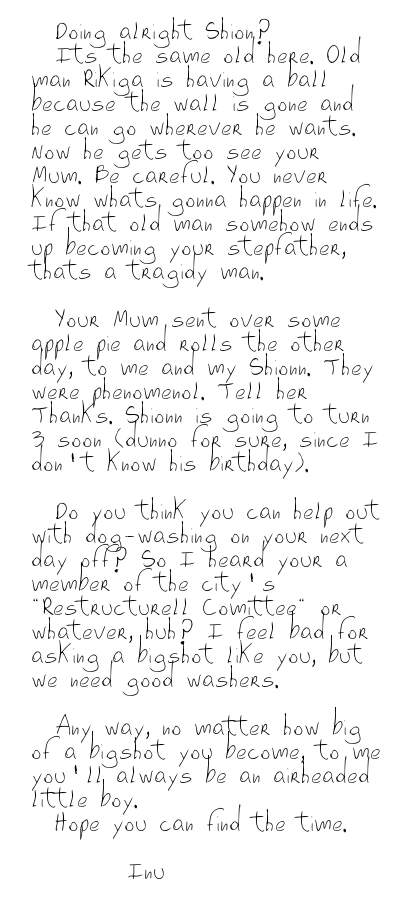
\includegraphics{OEBPS/Images/memo10.png}\\

Shion carefully folded the letter scribbled on rough paper, and put it
away. I'm going, Inukashi.

Cheep-cheep-cheep!

Tsukiyo cried at his feet. This mouse had chosen to remain by Shion's
side. He was a little older now, but was as energetic and bright as
ever. Karan was his absolute favourite person, and he slept in her bed
at night.

Another letter was from someone Shion had not dreamed of receiving word
from. It was from Sasori, the man in the underground realm. A few days
ago, Shion had been paid a visit by a sewer rat carrying the letter in
its mouth. In it was written a short message of thanks.

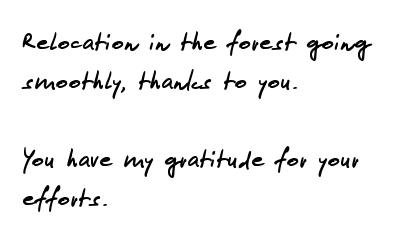
\includegraphics{OEBPS/Images/memo11.png}\\

Following the destruction of the Correctional Facility, the people of
the underground realm had fled into the forest on Rou's orders.

Promise them a land where they can live in peace. Shion had forwarded
Rou's short message to the Restructural Committee, and gotten permission
to allocate a part of the northern forest to those people.

The land was on the outskirts of Mao, where the Forest People used to
live. The dense expanse of forest protected their eyes, which were
sensitive to bright sunlight because of the darkness they were
accustomed to. Shion had chosen this spot after much deliberation.

Rou chose to remain underground. He ended his life there, along with a
few elders.

The remains of the Correctional Facility have now become a park.
Inukashi mentioned that he took Shionn there to play sometimes.

\emph{Time ambles along.}

\emph{\\
}

\emph{Everything changes.}

\emph{\\
}

\emph{But I'll never forget.}

Shion got up, and stood by the window. He threw it wide open.

\emph{Come on in, Nezumi―just like you did that night.}

Only a breeze, thick with the scent of young leaves, blew at him in
return.

He kept waiting.

No. 6―a city by that name once existed here.

It had existed, once the epitome of human intelligence, a utopian
city-state.
